\documentclass[semifinal]{cpecmu}

%% This is a sample document demonstrating how to use the CPECMU
%% project template. If you are having trouble, see "cpecmu.pdf" for
%% documentation.

\projectNo{P002-2/66}
\acadyear{2023}

\titleTH{เพชฌฆาตแม่มด: เกมแนวสยองขวัญแบบผู้เล่นหลายคน}
\titleEN{Witch Hunter: A Multiplayer Horror Game}

\author{นายธนดล เดชประภากร}{Tanadol Deachprapakorn}{630610734}
\author{นายภูริช สีนวลแล}{Purich Seenaullae}{630610752}

\cpeadvisor{karn}
\cpecommittee{sakgasit}
\cpecommittee{patiwet}

%% Some possible packages to include:
\usepackage[final]{graphicx} % for including graphics
\usepackage{subcaption} % for subfigures
\usepackage{multirow} % for multirow cells in tables

%% Add bookmarks and hyperlinks in the document.
\PassOptionsToPackage{hyphens}{url}
\usepackage[colorlinks=true,allcolors=Blue4,citecolor=red,linktoc=all]{hyperref}
\def\UrlLeft#1\UrlRight{$#1$}

%% Needed just by this example, but maybe not by most reports
\usepackage{afterpage} % for outputting
\usepackage{pdflscape} % for landscape figures and tables. 

%% Some other useful packages. Look these up to find out how to use
%% them.
% \usepackage{natbib}    % for author-year citation styles
% \usepackage{txfonts}
% \usepackage{appendix}  % for appendices on a per-chapter basis
% \usepackage{xtab}      % for tables that go over multiple pages
% \usepackage{subfigure} % for subfigures within a figure
% \usepackage{pstricks,pdftricks} % for access to special PostScript and PDF commands
% \usepackage{nomencl}   % if you have a list of abbreviations

%% if you're having problems with overfull boxes, you may need to increase
%% the tolerance to 9999
\tolerance=9999

% \bibliographystyle{plain}
% \bibliographystyle{IEEEbib}

% \renewcommand{\topfraction}{0.85}
% \renewcommand{\textfraction}{0.1}
% \renewcommand{\floatpagefraction}{0.75}

%% Example for glossary entry
%% Need to use glossary option
%% See glossaries package for complete documentation.
\ifglossary
  \newglossaryentry{lorem ipsum}{
    name=lorem ipsum,
    description={derived from Latin dolorem ipsum, translated as ``pain itself''}
  }
\fi

%% Uncomment this command to preview only specified LaTeX file(s)
%% imported with \include command below.
%% Any other file imported via \include but not specified here will not
%% be previewed.
%% Useful if your report is large, as you might not want to build
%% the entire file when editing a certain part of your report.
% \includeonly{chapters/intro,chapters/background}

\begin{document}
\maketitle
\makesignature

\ifproject
\begin{abstractTH}
เพชฌฆาตแม่มด: เกมแนวสยองขวัญแบบผู้เล่นหลายคน พัฒนาขึ้นเพื่อนำเสนอเกมสยองขวัญที่ให้ความบันเทิง มีแรงบันดาลใจจากความเชื่อยุคกลางที่มีอยู่ว่า ปีศาจปลอมแปลงเป็นสัตว์ได้หลายชนิด อาศัยอยู่ในป่ารกร้าง ผู้เล่นจะต้องต่อสู้กัน ทั้งฝ่ายปราบแม่มดและแม่มด โดยทีมปราบแม่มดต้องทำงานร่วมกันเพื่อทำภารกิจ ส่วนแม่มดมีหน้าที่ขัดขวางฝั่งตรงข้าม มีความสามารถที่จะแปลงกายเป็นสัตว์เพื่ออำพรางและขัดขวางภารกิจได้ เกมนี้พัฒนาโดยใช้ Unreal Engine เพื่อให้ผู้เล่นได้สัมผัสประสบการณ์ที่สมจริงผ่านมุมมองบุคคลที่หนึ่ง
\end{abstractTH}

\begin{abstract}
Witch Hunter: A Multiplayer Horror Game is developed to present an entaining horror game. It is inspired by medieval beliefs that demons can disguise themselves as animals and live in the wilderness. Players must fight each other, with one side playing as a team of demon hunters and the other as the witch. The demon hunters must work together to complete their mission, while the witch has the ability to transform into animals to obstruct and interfere with the mission. The game is developed using the Unreal Engine to provide players with an immersive first-person perspective.
\end{abstract}
\iffalse
\begin{dedication}
This document is dedicated to all Chiang Mai University students.

Dedication page is optional.
\end{dedication}
\fi % \iffalse

\begin{acknowledgments}
โครงงานเรื่อง เพชฌฆาตแม่มด: เกมแนวสยองขวัญแบบผู้เล่นหลายคน จะไม่สามารถสำเร็จลุล่วงลงได้ ถ้าไม่ได้รับความกรุณาจาก ผศ.ดร.กานต์ ปทานุคม
อาจารย์ที่ปรึกษาที่ได้เสียสละเวลาให้คำแนะนำ และข้อเสนอแนะที่มีคุณค่ามากมายตลอดการพัฒนาโครงงานนี้ รวมถึงคณะกรรมการสอบโครงงานทุกท่าน รศ.ดร.ปฏิเวธ วุฒิสารวัฒนา
และ รศ.ดร.ศักดิ์กษิต ระมิงค์วงศ์​ ที่ได้ให้คำติชมและข้อเสนอแนะที่สำคัญ

ขอขอบคุณภาควิชาวิศวกรรมคอมพิวเตอร์ มหาวิทยาลัยเชียงใหม่ ที่ได้สนับสนุนความรู้และทรัพยาการให้สามารถทำโครงงานนี้ได้สำเร็จ

ขอขอบคุณเพื่อน ๆ ที่ได้มีส่วนร่วมในการทดสอบเกม Witch Hunter ตั้งแต่ตอนที่เล่นแทบไม่ได้จนกระทั่งเสร็จสมบูรณ์ ขอขอบคุณที่ได้ทดลองเล่น ให้คำแนะนำ กำลังใจ และข้อเสนอแนะที่สำคัญ

\acksign{2024}{3}{26}
\end{acknowledgments}%
\fi % \ifproject

\contentspage

\ifproject
\figurelistpage

\tablelistpage
\fi % \ifproject

% \abbrlist % this page is optional

% \symlist % this page is optional

% \preface % this section is optional


\pagestyle{empty}\cleardoublepage
\normalspacing \setcounter{page}{1} \pagenumbering{arabic} \pagestyle{cpecmu}

\chapter{\ifenglish Introduction\else บทนำ\fi}

\section{\ifenglish Project rationale\else ที่มาของโครงงาน\fi}
แนวเกมสยองขวัญเป็นแนวเกมที่ได้รับความนิยมในปัจจุบัน หลายเกมเป็นเกมแบบผู้เล่นคนเดียว ซึ่งสามารถมอบประสบการณ์ที่เร้าใจ น่ากลัว ให้กับผู้เล่น อีกทั้งยังทำให้ผู้เล่นมีประสบการณ์ร่วมที่ดี แต่ทว่าเกมแบบผู้เล่นคนเดียวขาดเรื่องการปฏิสัมพันธ์กับผู้เล่นคนอื่น ผู้เล่นไม่สามารถมีประสบการณ์ร่วมกับผู้อื่นได้ และเกมแบบผู้เล่นคนเดียวยังเน้นด้านการเล่าเรื่อง ซึ่งบ่อยครั้งผู้เล่นมักจะไม่กลับมาเล่นซ้ำใหม่ ทางผู้พัฒนาจึงสนใจที่จะพัฒนาเกมสยองขวัญที่อาศัยความร่วมมือของผู้เล่นสองคนในการฝ่าฟันอุปสรรคในรูปแบบที่เกมสยองขวัญแบบผู้เล่นคนเดียวทำไม่ได้ และดึงดูดให้ผู้เล่นสามารถสนุกกับการกลับมาเล่นซ้ำใหม่ได้

\section{\ifenglish Objectives\else วัตถุประสงค์ของโครงงาน\fi}
\begin{enumerate}
    \item พัฒนาเกมแนวสยองขวัญที่เน้นให้ผู้เล่นได้ ทดลองประสบการณ์การต่อสู้และการทำงานร่วมกัน ในทีมเพื่อต่อสู่กับปีศาจที่ปลอมแปลงเป็นสัตว์ต่าง ๆ ในป่ารกร้าง
    \item ใช้ Unreal Engine เป็นเครื่องมือในการ พัฒนาเกมเพื่อสร้าง ประสบการณ์ที่สมจริง และ น่าตื่นเต้นในการต่อสู้และการแก้ปัญหาในสภาพแวด-ล้อมที่ท้าทาย
    \item ทำให้ผู้เล่นได้รับประสบการณ์ที่สนุกสนาน และ ท้าทายในการเล่นเกมที่มีความลึกลับและความหลาก-หลายในเนื้อหาและการเล่น
\end{enumerate}

\section{\ifenglish Project scope\else ขอบเขตของโครงงาน\fi}

\subsection{\ifenglish Hardware scope\else ขอบเขตด้านฮาร์ดแวร์\fi}
\begin{enumerate}
    \item โปรแกรมสามารถรองรับตัวควบคุมได้สองช่องทาง (คีย์บอร์ดและเมาส์)
\end{enumerate}

\subsection{\ifenglish Software scope\else ขอบเขตด้านซอฟต์แวร์\fi}
\begin{enumerate}
    \item เกมสามารถเล่นได้ผ่านทางคอมพิวเตอร์ระบบปฏิบัติการ Windows 10 ขึ้นไปเท่านั้น
\end{enumerate}

\section{\ifenglish Expected outcomes\else ประโยชน์ที่ได้รับ\fi}

ผู้เล่นเกมตื่นเต้นและสนุกสนานกับการเล่นเกมนี้ร่วมกับผู้อื่น ส่งเสริมให้ผู้เล่นมีปฏิสัมพันธ์ที่ดีในการเล่นเกมนี้ร่วมกัน

\section{\ifenglish Software technology\else เทคโนโลยีด้านซอฟต์แวร์\fi}
\begin{enumerate}
    \item Unreal Engine: เกมเอนจินที่ใช้พัฒนาวิดีโอเกม
    \item Git LFS: ระบบจัดการ version ของการพัฒนาโปรแกรม
    \item Gitlab: ในการจัดเก็บ repository ของโปรเจค

\end{enumerate}

\section{\ifenglish Project plan\else แผนการดำเนินงาน\fi}

\begin{plan}{12}{2022}{3}{2024}
    \planitem{12}{2022}{03}{2023}{รวบรวมความต้องการของผู้เล่น}
    \planitem{12}{2022}{03}{2023}{ออกแบบวิธีการเล่น}
    \planitem{01}{2023}{03}{2023}{สร้างต้นแบบ}
    \planitem{03}{2023}{05}{2023}{พัฒนาและทดสอบต้นแบบ}
    \planitem{06}{2023}{06}{2023}{สร้างสรรค์งานศิลป์}
    \planitem{12}{2023}{02}{2024}{สร้างสรรค์งานศิลป์ (ต่อ)}
    \planitem{12}{2023}{03}{2024}{เขียนโปรแกรมส่วนการเล่น}
    \planitem{01}{2024}{03}{2024}{งานเสียงและดนตรีประกอบ}
    \planitem{02}{2024}{03}{2024}{ทดสอบเกม}
    \planitem{02}{2024}{03}{2024}{วัดและรายงานผล}
    \planitem{03}{2024}{03}{2024}{เขียนโปรแกรมส่วน UI}
\end{plan}

\section{\ifenglish Roles and responsibilities\else บทบาทและความรับผิดชอบ\fi}
\begin{enumerate}
    \item นายธนดล เดชประภากร หน้าที่: Gameplay design, Game programmer, Sound design, Testing
    \item นายภูริช สีนวลแล หน้าที่: Gameplay design, UI/UX designer, Testing
\end{enumerate}

\section{\ifenglish%
Impacts of this project on society, health, safety, legal, and cultural issues
\else%
ผลกระทบด้านสังคม สุขภาพ ความปลอดภัย กฎหมาย และวัฒนธรรม
\fi}

โปรแกรมนี้สามารถสร้างเสริมทักษะความร่วมมือ การสื่อสาร และการแก้ไขปัญหาเฉพาะหน้าพร้อมความบันเทิงควบคู่กัน

\chapter{\ifenglish Background Knowledge and Theory\else ทฤษฎีที่เกี่ยวข้อง\fi}

การทำโครงงาน เริ่มต้นด้วยการศึกษาค้นคว้า ทฤษฎีที่เกี่ยวข้อง หรือ งานวิจัย/โครงงาน ที่เคยมีผู้นำเสนอไว้แล้ว ซึ่งเนื้อหาในบทนี้ก็จะเกี่ยวกับการอธิบายถึงสิ่งที่เกี่ยวข้องกับโครงงาน เพื่อให้ผู้อ่านเข้าใจเนื้อหาในบทถัดๆ ไปได้ง่ายขึ้น

\section{เกมสยองขวัญแบบผู้เล่นหลายคนในตลาด}
\subsection{Dead Space 3}

Dead Space 3 เป็นเกมสยองขวัญที่ให้ผู้เล่นสามารถเล่นโดยใช้ความร่วมมือจากผู้เล่น 2 คน โดยต่อสู้กับ Necromorph โดยรวมแล้วเป็นเกมสยองขวัญเอาชีวิตรอดที่ตึงเครียดและน่าตื่นเต้นที่นำเสนอประสบการณ์ความร่วมมือที่สมจริง เรื่องราวที่น่าดึงดูด และกลไกการเล่นเกมที่หลากหลายเพื่อให้ผู้เล่นมีส่วนร่วมและลุ้นตาม \cite{DeadSpace3}


\subsection{Left 4 Dead 2}

Left 4 Dead 2 เป็นเกมสยองขวัญเอาชีวิตรอดจากโลกที่เต็มไปด้วยฝูงผีดิบ โดยเล่นด้วยกันได้ตั้งแต่ 1 ถึง 4 คน ผู้เล่นจะรับบทบาทเป็นผู้เอาชีวิตรอด มีอาวุธให้ผู้เล่นได้เลือกตามความถนัดของตน โดยรวมแล้วเป็นเกมยิงแบบร่วมมือที่รวดเร็วและเข้มข้น ซึ่งนำเสนอการผสมผสานระหว่างกลยุทธ์ การทำงานเป็นทีม และความสยองขวัญ ลุ้นระทึกเอาชีวิตรอด กับรูปแบบการเล่นที่น่าดึงดูดและตัวละครที่น่าจดจำ \cite{L4D2}



\subsection{Phasmophobia}

Phasmophobia เกมนี้ให้ผู้เล่นสวมบทบาทเป็นนักล่าผี และ รองรับผู้เล่นสูงสุด 4 คนที่ทำงานร่วมกันเพื่อสำรวจสถานที่และ รวบรวมหลักฐานเหตุการณ์เหนือธรรมชาติ โดยรวมแล้วเป็นเกมสยองขวัญที่ไม่เหมือนใครและน่าดึงดูด ซึ่งรวมเอาองค์ประกอบของการสืบสวน การเอาชีวิตรอด และการเล่นเกมแบบร่วมมือกัน เป็นเกมที่ต้องใช้การสื่อสาร การทำงานเป็นทีม และการคิดเชิงกลยุทธ์เพื่อให้ประสบความสำเร็จ \cite{Phasmophobia}


\subsection{The Forest}

The Forest เกมสยองขวัญเอาชีวิตรอด open world โดยผู้เล่นทำงานร่วมกันเพื่อสร้างที่พักพิง รวบรวมทรัพยากร และ ป้องกันมนุษย์กลายพันธุ์ โดยรวมแล้วเป็นเกมสยองขวัญเอาชีวิตรอดที่น่าตื่นเต้นและท้าทายที่นำเสนอการผสมผสานที่ไม่เหมือนใครระหว่างการสำรวจ การสร้าง และการต่อสู้ ด้วยบรรยากาศที่ตึงเครียด ศัตรูที่ท้าทาย และโลกที่สมจริง \cite{TheForest}



\subsection{Devour}

Devour เป็นเกมสยองขวัญเอาชีวิตรอดแบบอาศัยความร่วมมือของผู้เล่น 1-4 คน แต่ละเกมยาวหนึ่งชั่วโมง หน้าที่ของผู้เล่น คือ ทำภารกิจในรูปแบบต่าง ๆ เพื่อเอาตัวรอดจากสมาชิกลัทธิที่ถูกผีสิง เช่น การเผาแพะเพื่อทำพิธีกรรม โดยผู้เล่นจะต้องรวบรวมทรัพยากรต่าง ๆ เพื่อใช้ในการทำภารกิจ และต้องระวังศัตรูที่อยู่รอบตัว \cite{Devour}

\section{เครื่องมือที่ใช้ในการพัฒนา}
\subsection{Unreal Engine 5}
Unreal Engine 5 เป็นเครื่องมือพัฒนาเกมและซอฟต์แวร์สำหรับสร้างสภาพแวดล้อมแบบสามมิติ (3D) ที่ถูกพัฒนาโดย Epic Games ซึ่งเป็นบริษัทผู้พัฒนาเกมระดับโลกและเจ้าของหรือผู้จัดการสิทธิบัตรของหลายแพลตฟอร์มเกมที่สำคัญ เช่น Fortnite และ Gears of War Unreal Engine 5 เป็นเวอร์ชันล่าสุดของเครื่องมือการพัฒนาเกมของค่ายนี้และถูกประกาศเปิดตัวครั้งแรกในปี 2020

\subsection{Blender}
Blender เป็นโปรแกรมซอฟต์แวร์สำหรับสร้างกราฟิก 3 มิติ (3D) ที่มีความสามารถหลากหลาย เช่น การออกแบบและสร้างโมเดล 3 มิติ, การทำแอนิเมชัน, การสร้างภาพนิ่ง, และการสร้างภาพเคลื่อนไหว (วิดีโอ) ซึ่งมีความยืดหยุ่นและมีฟังก์ชันมากมายที่ช่วยให้นักออกแบบสามารถสร้างงานศิลปะที่มีคุณภาพสูงได้ โดย \\Blender เป็นโปรแกรมฟรีและเปิดตัวสำหรับใช้งาน มันสามารถใช้ได้กับหลายแพลตฟอร์ม เช่น Windows, macOS, และ Linux และมีชุดเครื่องมือที่ครอบคลุมตั้งแต่การสร้างโมเดลจนถึงการนำเสนองานออกมาในรูปแบบที่ต้องการได้ โดยสามารถนำผลงานที่สร้างขึ้นใน Blender ไปใช้ในหลายอุตสาหกรรม เช่น ภาพยนตร์, การทำเกม, การออกแบบผลิตภัณฑ์, และการพิมพ์ 3 มิติ

\subsection{GitLFS}
GitLFS ย่อมาจาก Git Large File Storage ซึ่งเป็นระบบการจัดการไฟล์ขนาดใหญ่ใน Git โดยเฉพาะ ซึ่ง Git นั้นเป็นระบบควบคุมเวอร์ชัน (Version Control System) ที่ใช้สำหรับการจัดการโค้ด ซึ่งมักจะใช้ในการพัฒนาซอฟต์แวร์ แต่มันไม่ได้เหมาะสำหรับการจัดเก็บไฟล์ขนาดใหญ่ เช่น ไฟล์เสียงวิดีโอหรือไฟล์ภาพที่มีขนาดใหญ่มาก
GitLFS ถูกพัฒนาขึ้นเพื่อแก้ไขปัญหานี้ โดย GitLFS ช่วยในการจัดเก็บไฟล์ขนาดใหญ่ในเครื่องเซิร์ฟเวอร์อย่างมีประสิทธิภาพ โดยไม่ทำให้เครื่องเซิร์ฟเวอร์โหลดไฟล์ทั้งหมดเมื่อมีการดึงโค้ดที่มีไฟล์ขนาดใหญ่จาก Git repository แทนที่จะเก็บไฟล์โดยตรงใน repository เช่นเดียวกับไฟล์ทั่วไป GitLFS จะเก็บไฟล์ขนาดใหญ่ในพื้นที่ที่เรียกว่า LFS storage ซึ่งส่วนใหญ่จะอยู่ในเครื่องเซิร์ฟเวอร์ภายนอก
การใช้ GitLFS ช่วยลดขนาดของ Git repository ช่วยในการจัดการไฟล์ขนาดใหญ่ที่มีการเปลี่ยนแปลงบ่อย ๆ และทำให้การทำงานร่วมกันในโปรเจกต์ที่มีไฟล์ขนาดใหญ่เป็นไปอย่างมีประสิทธิภาพมากขึ้น

\subsection{GitLab}
GitLab เป็นแพลตฟอร์มการพัฒนาซอฟต์แวร์ที่ให้บริการเครื่องมือต่างๆ ที่เกี่ยวข้องกับการจัดการโครงการพัฒนาซอฟต์แวร์ ซึ่งรวมถึงระบบควบคุมเวอร์ชัน Git ระบบติดตามปัญหา (Issue Tracking System) ระบบวิกิ (Wiki System) และระบบการดำเนินการต่าง ๆ ที่เกี่ยวข้องกับการพัฒนาซอฟต์แวร์และการทำงานในโครงการซอฟต์แวร์
นอกจากนี้ GitLab ยังเป็นเครื่องมือที่ให้บริการพื้นที่เก็บโค้ด (Repository Hosting Service) และให้บริการต่าง ๆ เกี่ยวกับการจัดการ Source Code เช่น การสร้างและจัดการซอร์สโค้ด การจัดการเวอร์ชันของโค้ด การเปิดเผยโค้ดต่าง ๆ Collaborative Coding การตรวจสอบโค้ด (Code Review) และการจัดการเครื่องมือต่าง ๆ ที่เกี่ยวข้องกับการพัฒนาซอฟต์แวร์ ทำให้ GitLab เป็นอีกทางเลือกหนึ่งสำหรับทีมที่ต้องการจัดการโครงการพัฒนาซอฟต์แวร์ของตน
นอกจาก GitLab Community Edition ที่เป็นเวอร์ชันโอเพ่นซอร์ส (Open Source) แล้ว ยังมี GitLab Enterprise Edition ที่เป็นเวอร์ชันเสียเงินที่มีฟีเจอร์เพิ่มเติมที่เหมาะสำหรับองค์กรหรือธุรกิจที่ต้องการระบบควบคุมเวอร์ชันของตนเองและความมั่นคงของการให้บริการ

\subsection{Mixamo}
Mixamo เป็นบริการออนไลน์ที่เชื่อมโยงกับ Adobe Creative Cloud ที่มุ่งเน้นการสร้างและปรับแต่งตัวละครแบบ 3 มิติ (3D characters) และการทำแอนิเมชัน (animation) อย่างรวดเร็วและง่ายดาย ในช่วงเวลาที่ผ่านมา Mixamo เป็นที่นิยมในวงการเกมและอินเตอร์เน็ตเพราะการใช้งานที่สะดวกและประหยัดเวลา โดยเฉพาะสำหรับนักพัฒนาเกม ซึ่งสามารถนำตัวละครและแอนิเมชันจาก Mixamo ไปใช้ในโปรเจกต์เกมของตนได้.

\subsection{Character Creator}
Character Creator เป็นซอฟต์แวร์ที่ใช้สร้างตัวละครสามมิติ (3D characters) ที่มีความสมจริงสำหรับใช้ในเกม ภาพนิ่ง หรือวิดีโออนิเมชัน ซอฟต์แวร์นี้ถูกพัฒนาโดย Reallusion และมีความสามารถที่ให้ผู้ใช้สร้างตัวละครที่หลากหลายในแง่มุมต่า งๆ ซึ่งรวมถึงรายละเอียดที่มากมาย เช่น รูปร่างของร่างกาย สีผิว ทรงผม ส่วนสวมใส่ และอื่น ๆ ที่เกี่ยวข้องกับลักษณะภายนอกของตัวละคร
Character Creator มีเครื่องมือที่ทำให้การสร้างตัวละครในระดับที่มีความสมจริงสูงมากขึ้น โดยสามารถปรับแต่งรายละเอียดต่างๆ ของตัวละครได้อย่างอิสระ เช่น การปรับแต่งรูปร่าง, สีผิว, ทรงผม, สร้างเสื้อผ้าและอุปกรณ์ต่างๆ เพื่อให้ตัวละครมีความเป็นเอกลักษณ์และสอดคล้องกับความต้องการของโครงการ
นอกจากนี้ Character Creator ยังมีการใช้งานร่วมกับโปรแกรมอื่นๆ เช่น Maya, Blender, Unity, และ Unreal Engine เพื่อให้ผู้ใช้สามารถนำเข้าตัวละครที่สร้างขึ้นมาใช้ในโปรเจกต์พัฒนาซอฟต์แวร์ต่าง ๆ ได้อย่างสะดวกสบาย ทำให้เป็นเครื่องมือที่มีประสิทธิภาพและความสามารถในการสร้างตัวละครสามมิติที่มีคุณภาพสูง


\section{\ifenglish%
\ifcpe CPE \else ISNE \fi knowledge used, applied, or integrated in this project
\else%
ความรู้ตามหลักสูตรซึ่งถูกนำมาใช้หรือบูรณาการในโครงงาน
\fi
}

\begin{enumerate}
  \item Software Engineering: ใช้ความรู้เรื่องการจัดการการพัฒนาซอฟต์แวร์
  \item Computer Networking: ใช้ความรู้ในเรื่องเครือข่ายคอมพิวเตอร์ในการพัฒนาส่วนการเล่นหลายคน
  \item Object-oriented Programming: ใช้ความรู้ในการเขียนโปรแกรมเชิงวัตถุในการเขียนโปรแกรม
\end{enumerate}


\section{\ifenglish%
Extracurricular knowledge used, applied, or integrated in this project
\else%
ความรู้นอกหลักสูตรซึ่งถูกนำมาใช้หรือบูรณาการในโครงงาน
\fi
}


\begin{enumerate}
  \item การพัฒนาเกมด้วย Unreal Engine โดยใช้ Blueprint และภาษา C++
  \item การออกแบบวิธีการเล่นและฉาก
  \item การออกแบบงานศิลป์ในเกม
  \item การสร้างเนื้อเรื่องและเนื้อหาในเกม
\end{enumerate}


\chapter{\ifproject%
\ifenglish Project Structure and Methodology\else โครงสร้างและขั้นตอนการทำงาน\fi
\else%
\ifenglish Project Structure\else โครงสร้างของโครงงาน\fi
\fi
}

ในบทนี้จะกล่าวถึงหลักการ และการออกแบบระบบ

\makeatletter

% \renewcommand\section{\@startsection {section}{1}{\z@}%
%                                    {13.5ex \@plus -1ex \@minus -.2ex}%
%                                    {2.3ex \@plus.2ex}%
%                                    {\normalfont\large\bfseries}}

\makeatother
%\vspace{2ex}
% \titleformat{\section}{\normalfont\bfseries}{\thesection}{1em}{}
% \titlespacing*{\section}{0pt}{10ex}{0pt}

\section{เนื้อหา}

\subsection{เนื้อเรื่อง}

เกมนี้มีเนื่อเรื่องและสถานที่อยู่ในยุโรปยุคกลาง ตามความเชื่อที่ว่า ปีศาจสามารถปลอมแปลงเป็นสัตว์ชนิด
หนึ่ง อาศัยอยู่ในป่ารกร้าง หน้าที่ของผู้เล่นคือ ต้องไปปราบปีศาจร้ายและทําให้ผู้คนปลอดภัย

\subsection{ดนตรีและเสียงประกอบ}

เกมนี้มีเสียงประกอบที่สร้างความสมจริงและความสยองขวัญ โดยมีเสียงประกอบทั้งหมด 2 ชนิด ได้แก่ ดนตรี ซาวด์เอฟเฟค
\begin{itemize}
  \item เสียงดนตรี: ถูกเล่นเมื่อผู้เล่นเห็นฝั่งตรงข้ามหรือโจมตีกัน โดยเป็นเสียงดนตรีที่สร้างความระทึก และหยุดเล่นเมื่อผู้เล่นหลบหนีไปห่างจากฝั่งตรงข้าม
  \item เสียงซาวด์เอฟเฟค: ถูกเล่นเมื่อผู้เล่นทำการกระทำต่าง ๆ
\end{itemize}

เสียงซาวด์เอฟเฟคเป็นเสียงแบบ 3 มิติที่มีระยะการได้ยินที่เหมาะสม ซึ่งทำให้ผู้เล่นสามารถระบุตำแหน่งของผู้เล่นคนอื่น ๆ ได้ 
นอกจากนี้แล้วเสียงซาวน์เอฟเฟคการเดินและวิ่งจะขึ้นอยู่กับพื้นผิวที่ผู้เล่นกำลังเคลื่อนที่อยู่เพื่อความสมจริง

\subsection{ฉาก}

สถานที่ของเกมคือป่าสนแห้งแล้งแห่งหนึ่งในยุโรป ดังแสดงในรูปที่ ~\ref{fig:Map} และ ~\ref{fig:atmosphere}  ขนาดของแผนที่ คือ 400 x 400 เมตร ประกอบไปด้วยทะเลสาบ 
น้ำตก ลำธาร ป่าสน และเนินเขา รวมถึงมีบ้านเก่า ๆ ที่ถูกทิ้งไว้ ซึ่งสามารถเป็นจุดนัดพบได้ เวลาของเกมคือช่วงกลางคืน 
สถานที่นอกจากมืดแล้วยังมีหมอกหนา ทำให้มองเห็นได้ไม่ชัดเจน เพื่อเพิ่มความระทึกให้กับผู้เล่น

\begin{figure}[p]
  \begin{center}
  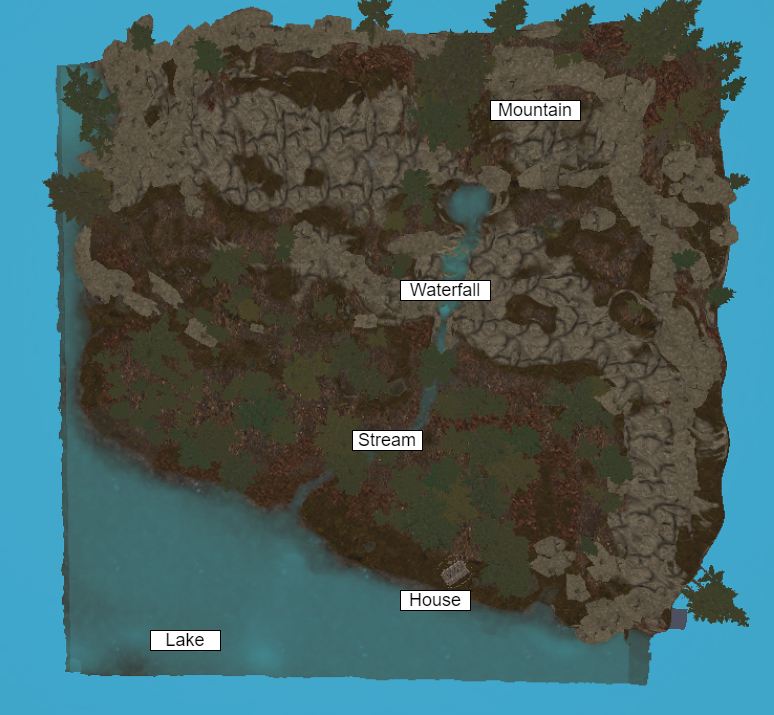
\includegraphics[width=0.7\textwidth]{./img/scene/WitchHunter-Map.png}
  \end{center}
  \caption[ภาพมุมสูงแสดงตำแหน่งของสถานที่ต่าง ๆ
  และภูมิประเทศของฉากในเกม]{ภาพมุมสูงแสดงตำแหน่งของสถานที่ต่าง ๆ
  และภูมิประเทศของฉากในเกม}
  \label{fig:Map}
\end{figure}

\begin{figure}[p]
  \begin{center}
  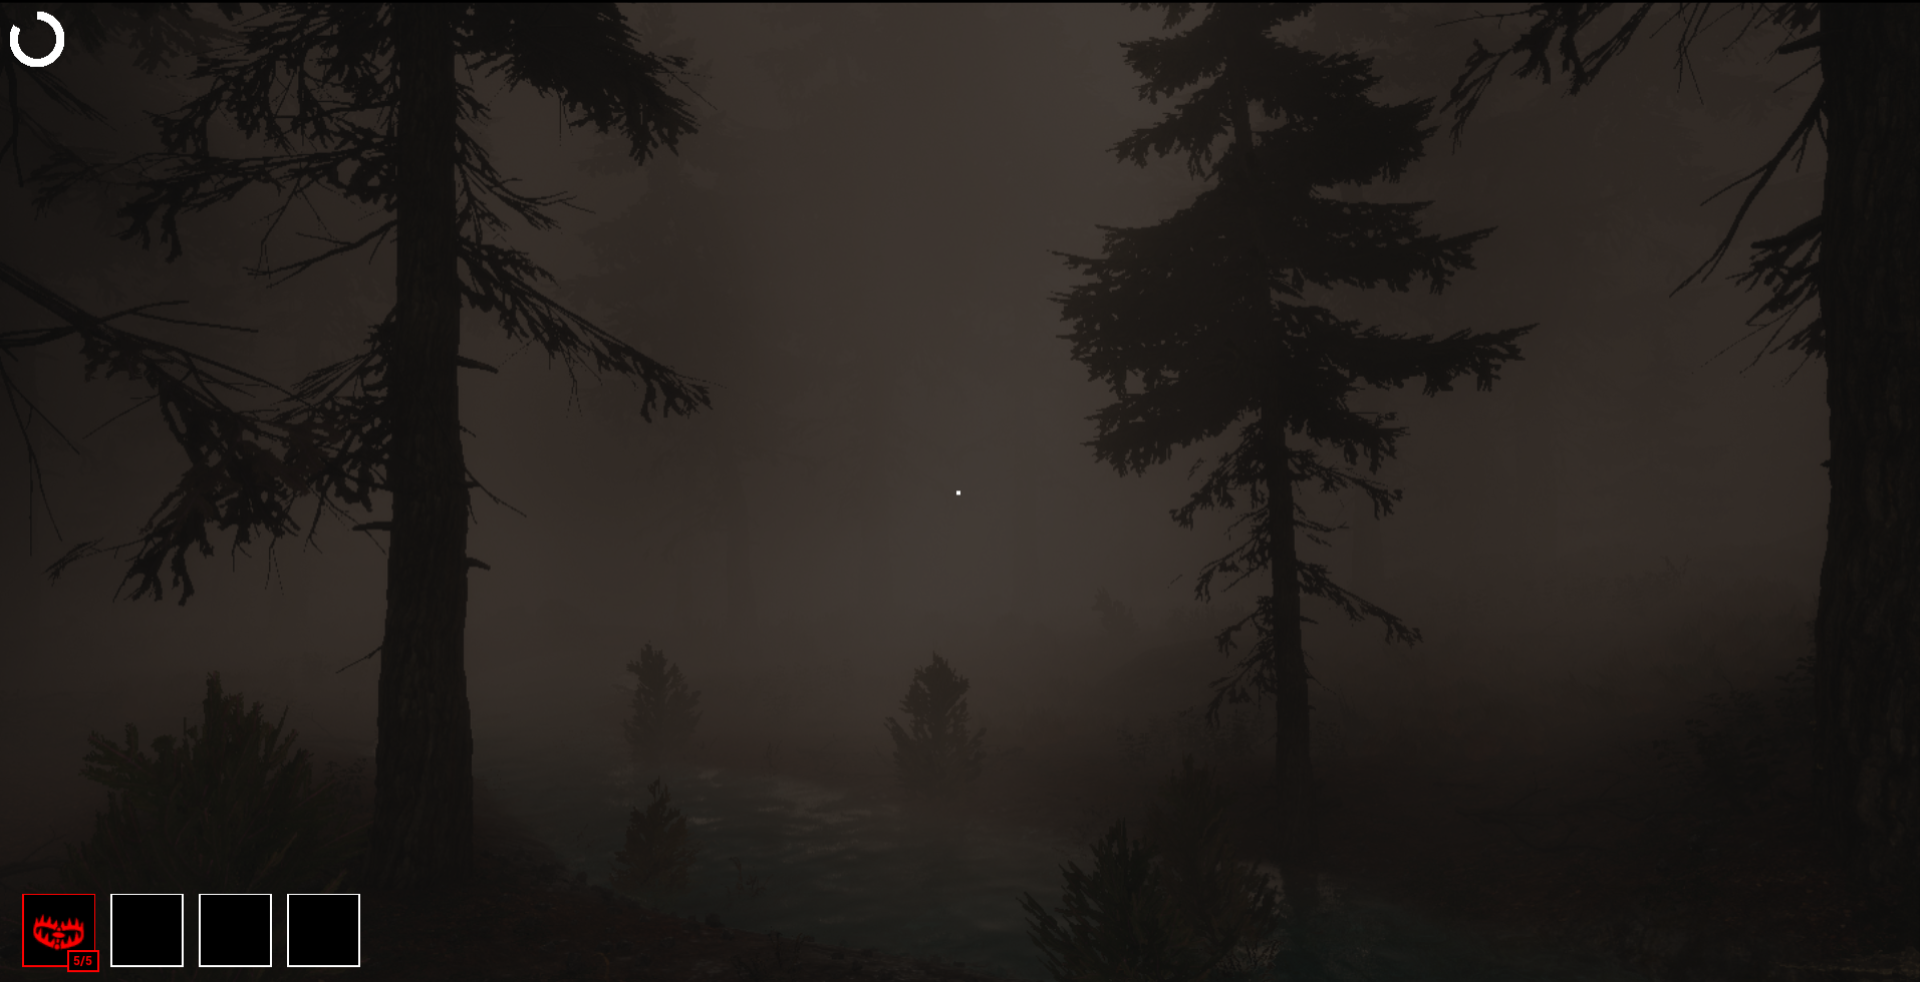
\includegraphics[width=\textwidth]{./img/scene/atmosphere.png}
  \end{center}
  \caption[ภาพบรรยากาศภายในเกม]{ภาพบรรยากาศภายในเกม}
  \label{fig:atmosphere}
\end{figure}

\subsection{ตัวละคร}

ในเกมนี้มีตัวละครทั้งหมด 3 ตัว ได้แก่ 2 ตัวของฝ่าย Hunters และ 1 ตัวของฝ่าย Witch ตัวละครถูกสร้างขึ้นโดยดัดแปลงจากโมเดลเสื้อผ้าและร่างกายที่มีอยู่แล้วในโปรแกรม Reallusion Character Creator

\subsubsection{ตัวละครฝ่าย Hunters}

แบ่งเป็น 2 ตัวละคร ชายและหญิง ซึ่งเป็นนายพรานและมีความสามารถเหมือนกันทั้งคู่ ดังแสดงในรูปที่ ~\ref{fig:emma} และ ~\ref{fig:eric}

\begin{figure}
  \centering
  \begin{subcaptionblock}{.4\textwidth}
    \centering
    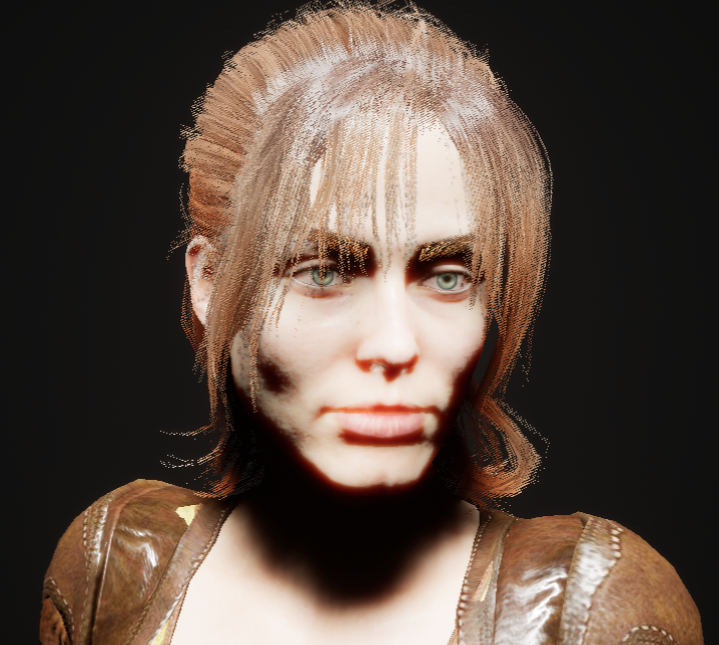
\includegraphics[width=.8\linewidth]{./img/characters/emma_face.png}
    \caption{ภาพใบหน้าตัวละคร Hunter หญิง}\label{ภาพใบหน้าตัวละคร Hunter หญิง}
  \end{subcaptionblock}%
  \begin{subcaptionblock}{.4\textwidth}
    \centering
    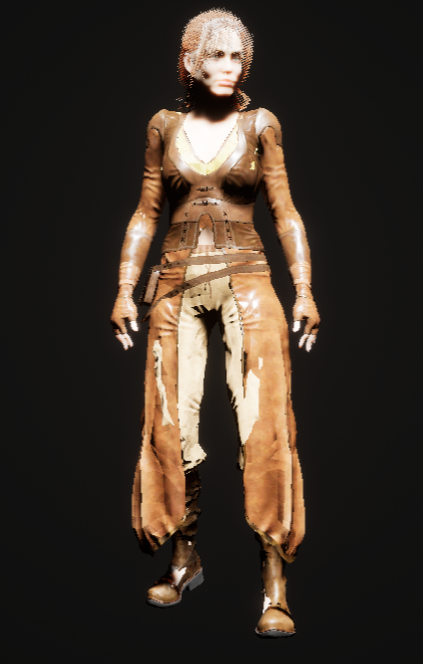
\includegraphics[width=.8\linewidth]{./img/characters/emma_full.png}
    \caption{ภาพเต็มตัวตัวละคร Hunter หญิง}\label{ภาพตัวเต็มตัวละคร Hunter หญิง}
  \end{subcaptionblock}%
  \caption{ภาพตัวละคร Hunter หญิง}\label{fig:emma}
\end{figure}

\begin{figure}
  \centering
  \begin{subcaptionblock}{.4\textwidth}
    \centering
    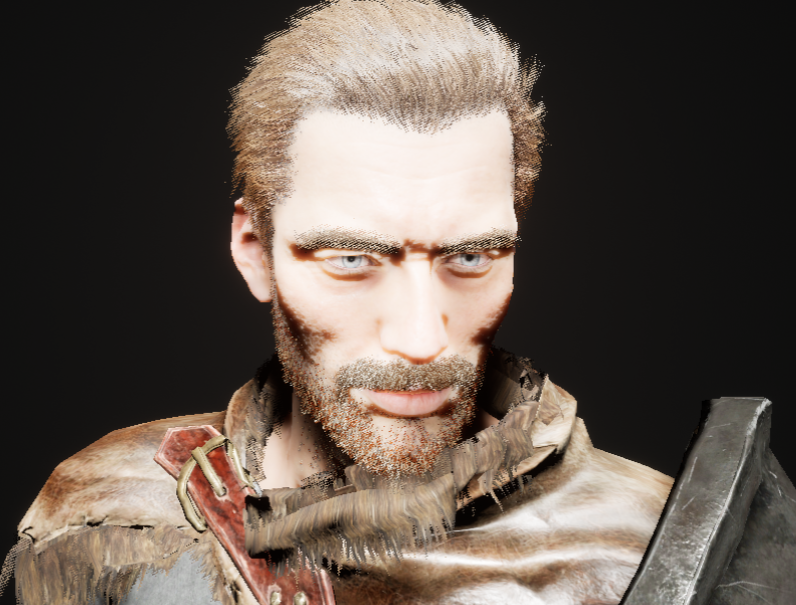
\includegraphics[width=.8\linewidth]{./img/characters/eric_face.png}
    \caption{ภาพใบหน้าตัวละคร Hunter ชาย}\label{ภาพใบหน้าตัวละคร Hunter ชาย}
  \end{subcaptionblock}%
  \begin{subcaptionblock}{.4\textwidth}
    \centering
    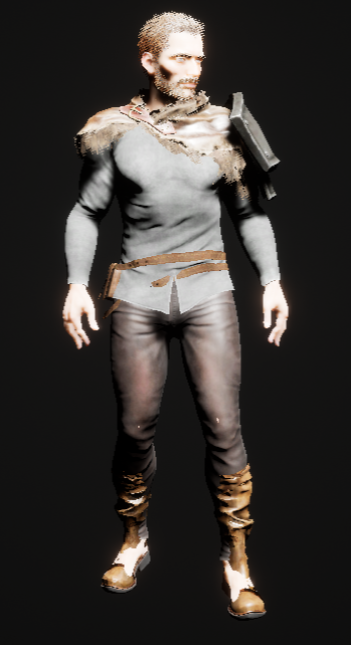
\includegraphics[width=.8\linewidth]{./img/characters/eric_full.png}
    \caption{ภาพเต็มตัวตัวละคร Hunter ชาย}\label{ภาพตัวเต็มตัวละคร Hunter ชาย}
  \end{subcaptionblock}%
  \caption{ภาพตัวละคร Hunter ชาย}\label{fig:eric}
\end{figure}

\subsubsection{ตัวละครฝ่าย Witch}

ร่างของแม่มดจะเป็นหญิงแก่หน้าตาอัปลักษณ์ที่มีศีรษะหันไปด้านหลังและเดินถอยหลัง ดังแสดงในรูปที่ ~\ref{fig:witch}

\begin{figure}
  \centering
  \begin{subcaptionblock}{.4\textwidth}
    \centering
    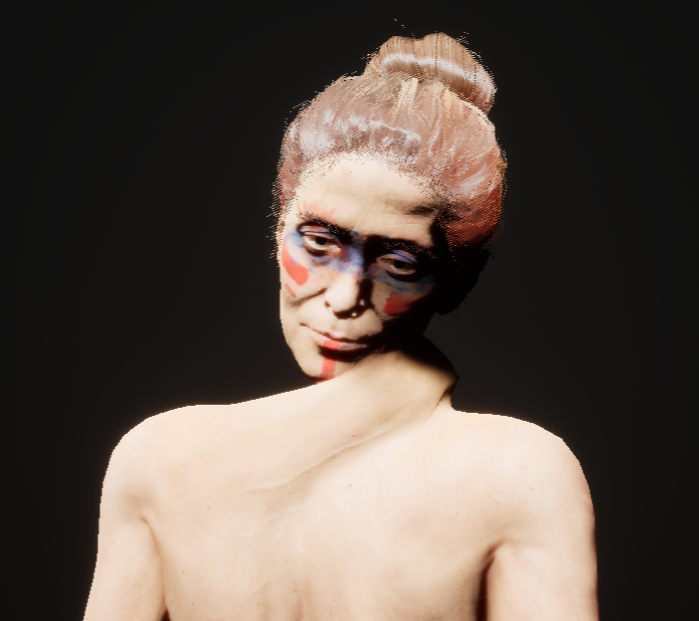
\includegraphics[width=.8\linewidth]{./img/characters/witch_face.png}
    \caption{ภาพใบหน้าตัวละคร Witch}\label{ภาพใบหน้าตัวละคร Witch}
  \end{subcaptionblock}%
  \begin{subcaptionblock}{.4\textwidth}
    \centering
    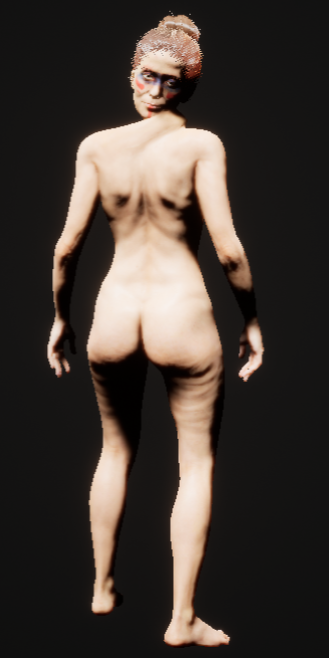
\includegraphics[width=.8\linewidth]{./img/characters/witch_full.png}
    \caption{ภาพเต็มตัวตัวละคร Witch}\label{ภาพตัวเต็มตัวละคร Witch}
  \end{subcaptionblock}%
  \caption{ภาพตัวละคร Witch}\label{fig:witch}
\end{figure}

\begin{figure}[p]
  \begin{center}
  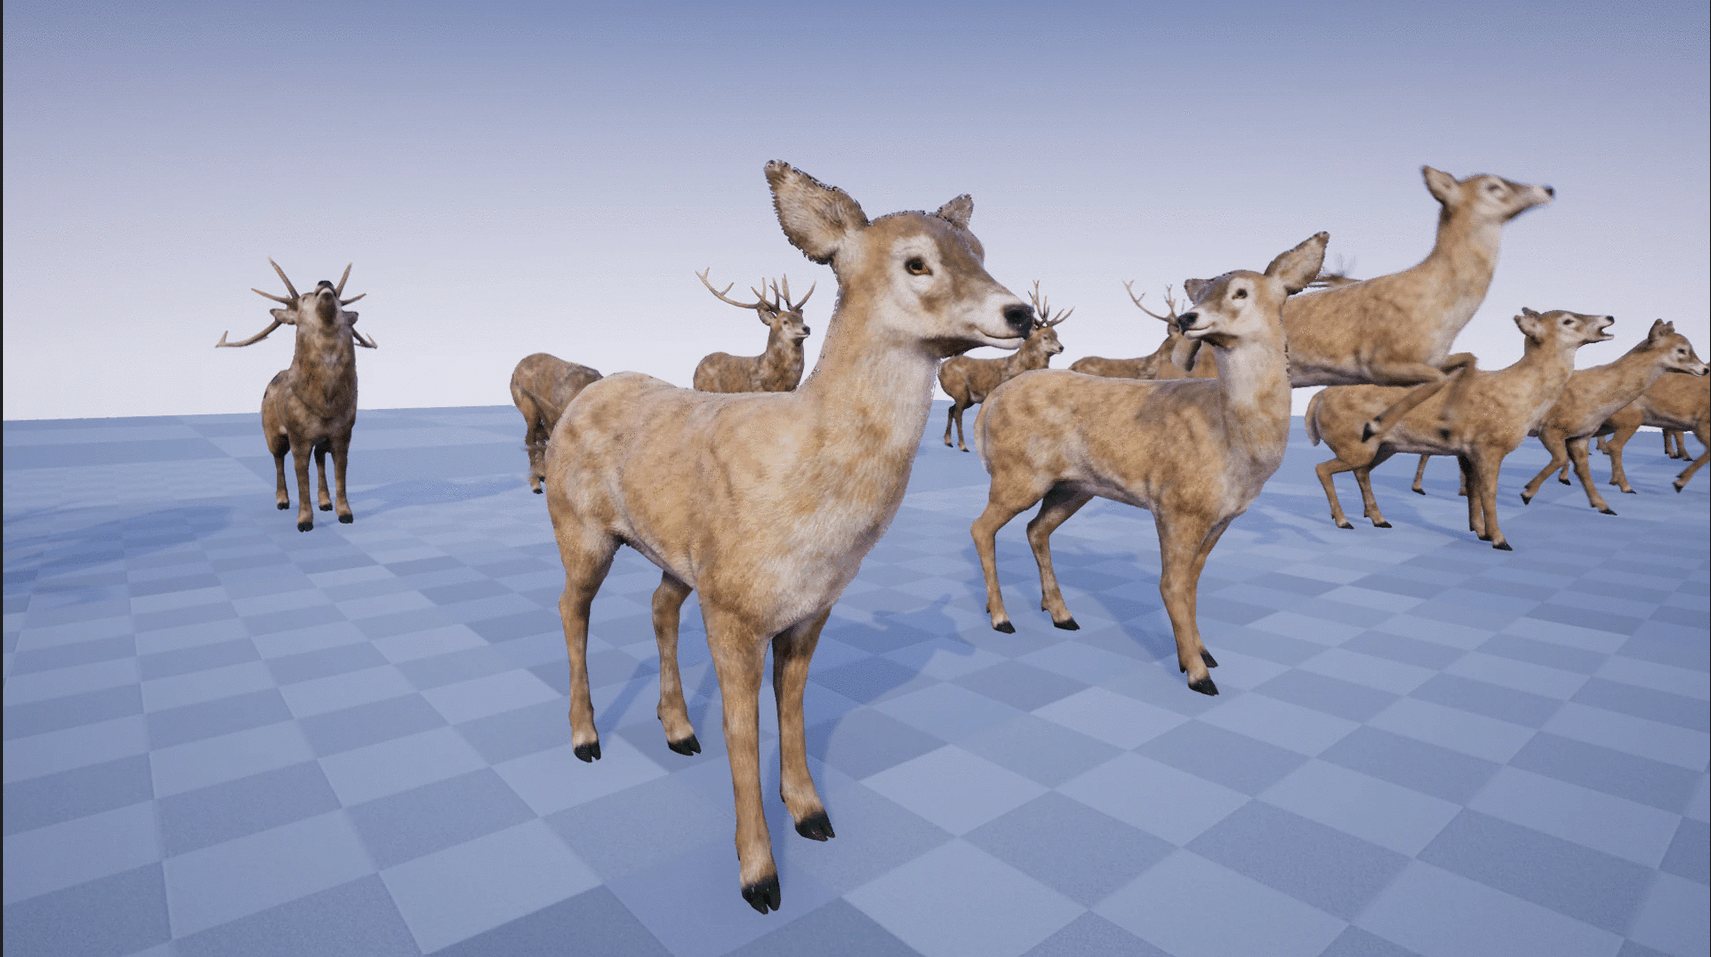
\includegraphics[width=\textwidth]{./img/characters/deerdoe.png}
  \end{center}
  \caption[ภาพตัวละครกวาง]{ภาพตัวละครกวาง}
  \label{fig:deer}
\end{figure}

\subsubsection{ตัวละครกวาง}

กวางสามารถนอน กิน และเดินไปมาได้ อีกทั้งยังสามารถวิ่งหนี Hunter ที่พยายามจับได้อีกด้วย นอกเหนือจากนี้แล้วกวางยังสามารถถูกควบคุมได้โดย Witch เพื่อหลอกล่อ Hunter

\section{วิธีการเล่น}

เพชฌฆาตแม่มด (Witch Hunter) เป็นเกมสยองขวัญแบบหลายผู้เล่น 2vs1 โดยผู้เล่นแบ่งออกเป็น 2 ฝั่ง 
ฝั่งของ Hunters ประกอบด้วยผู้เล่น 2 คน ต้องร่วมมือกันทำภารกิจที่กำหนดไว้ ซึ่งก็คือการจับกวางที่เป็นลูกสมุนของแม่มด 
แล้วนำเลือดกวางมาทำพิธี 6 ครั้งตามจุดที่กำหนดไว้แบบสุ่ม ในขณะที่ฝั่ง Witch ซึ่งประกอบด้วยผู้เล่น 1 คน
ต้องขัดขวางและถ่วงเวลาฝ่าย Hunters ไม่ให้ทำภารกิจสำเร็จ โดยการปลอมตัวเป็นกวางเพื่อหลอกล่อ Hunters และทำการโจมตีด้วยเวทมนต์

\subsection{การเล่นของฝ่าย Hunters}

\subsubsection{การจับกวาง}

สามารถจับกวางด้วยการปามีดศักดิ์สิทธิ์หรือวางกับดักทิ้งไว้ ดังแสดงในรูปที่ ~\ref{fig:การจับกวางโดยใช้มีด} และ ~\ref{fig:trap} ตามลำดับ เมื่อกวางถูกโจมตีหรือถูกกับดักจะล้มลง Hunter มีหน้าที่ที่ต้องทำการสกัดเลือดจากตัวกวางที่ล้มลงไปตามรูปที่ ~\ref{fig:blood}
กวางแต่ละตัวไม่ได้นิ่งเฉย แต่สามารถนอน กิน หรือเดินไปมาได้ ซึ่ง
Hunter ต้องอาศัยความละมุมละม่อมในการจับกวางเพราะถ้าหากวิ่งเข้าไปหาหรือเดินเข้าไปใกล้เกินไป กวางจะตกใจ
วิ่งหนี ทำให้อีกฝั่งอาจสังเกตุเห็นความผิดปกตินี้และสามารถระบุตำแหน่งของ Hunter ได้

\begin{figure}[h]
  \begin{center}
  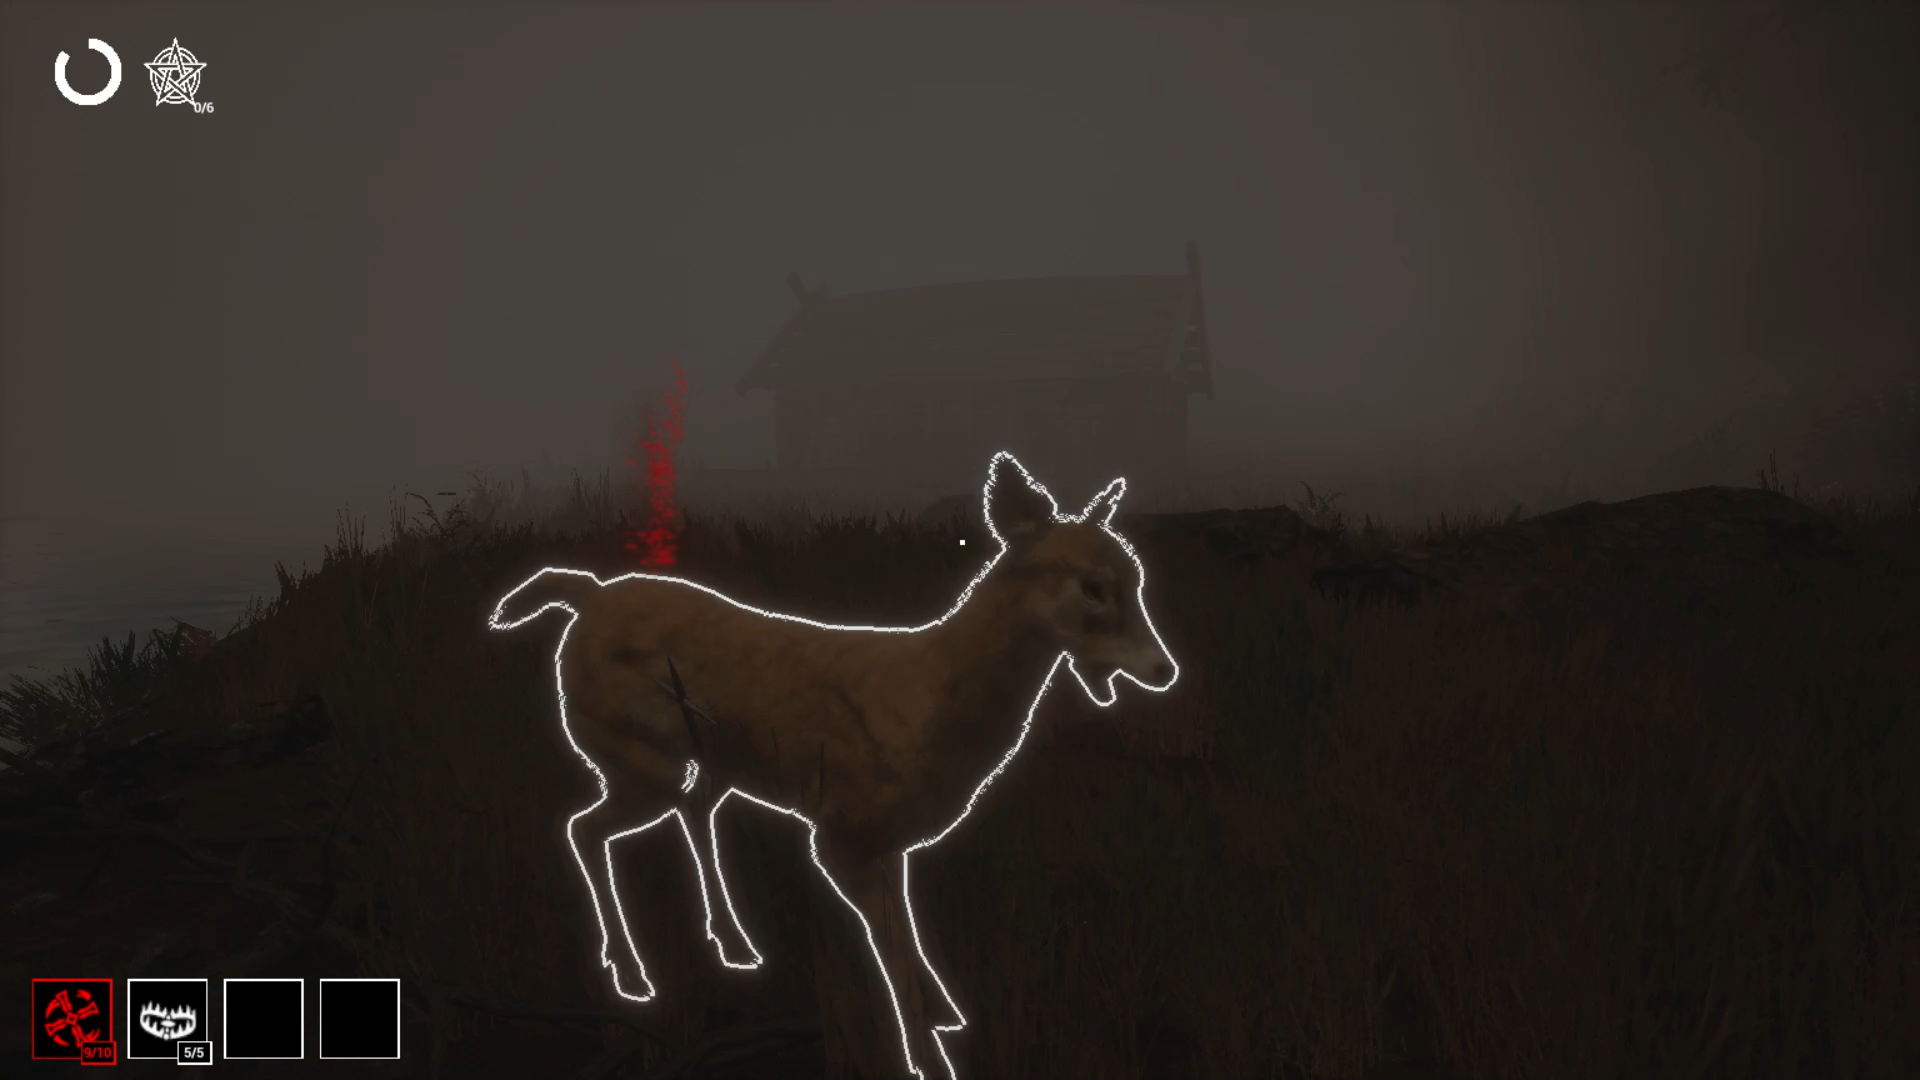
\includegraphics[width=\textwidth]{./img/mechanics/throw_knife_deer.png}
  \end{center}
    \caption[การจับกวางโดยใช้มีด]{การจับกวางโดยใช้มีด}
    \label{fig:การจับกวางโดยใช้มีด}
\end{figure}

\begin{figure}[p]
  \begin{center}
  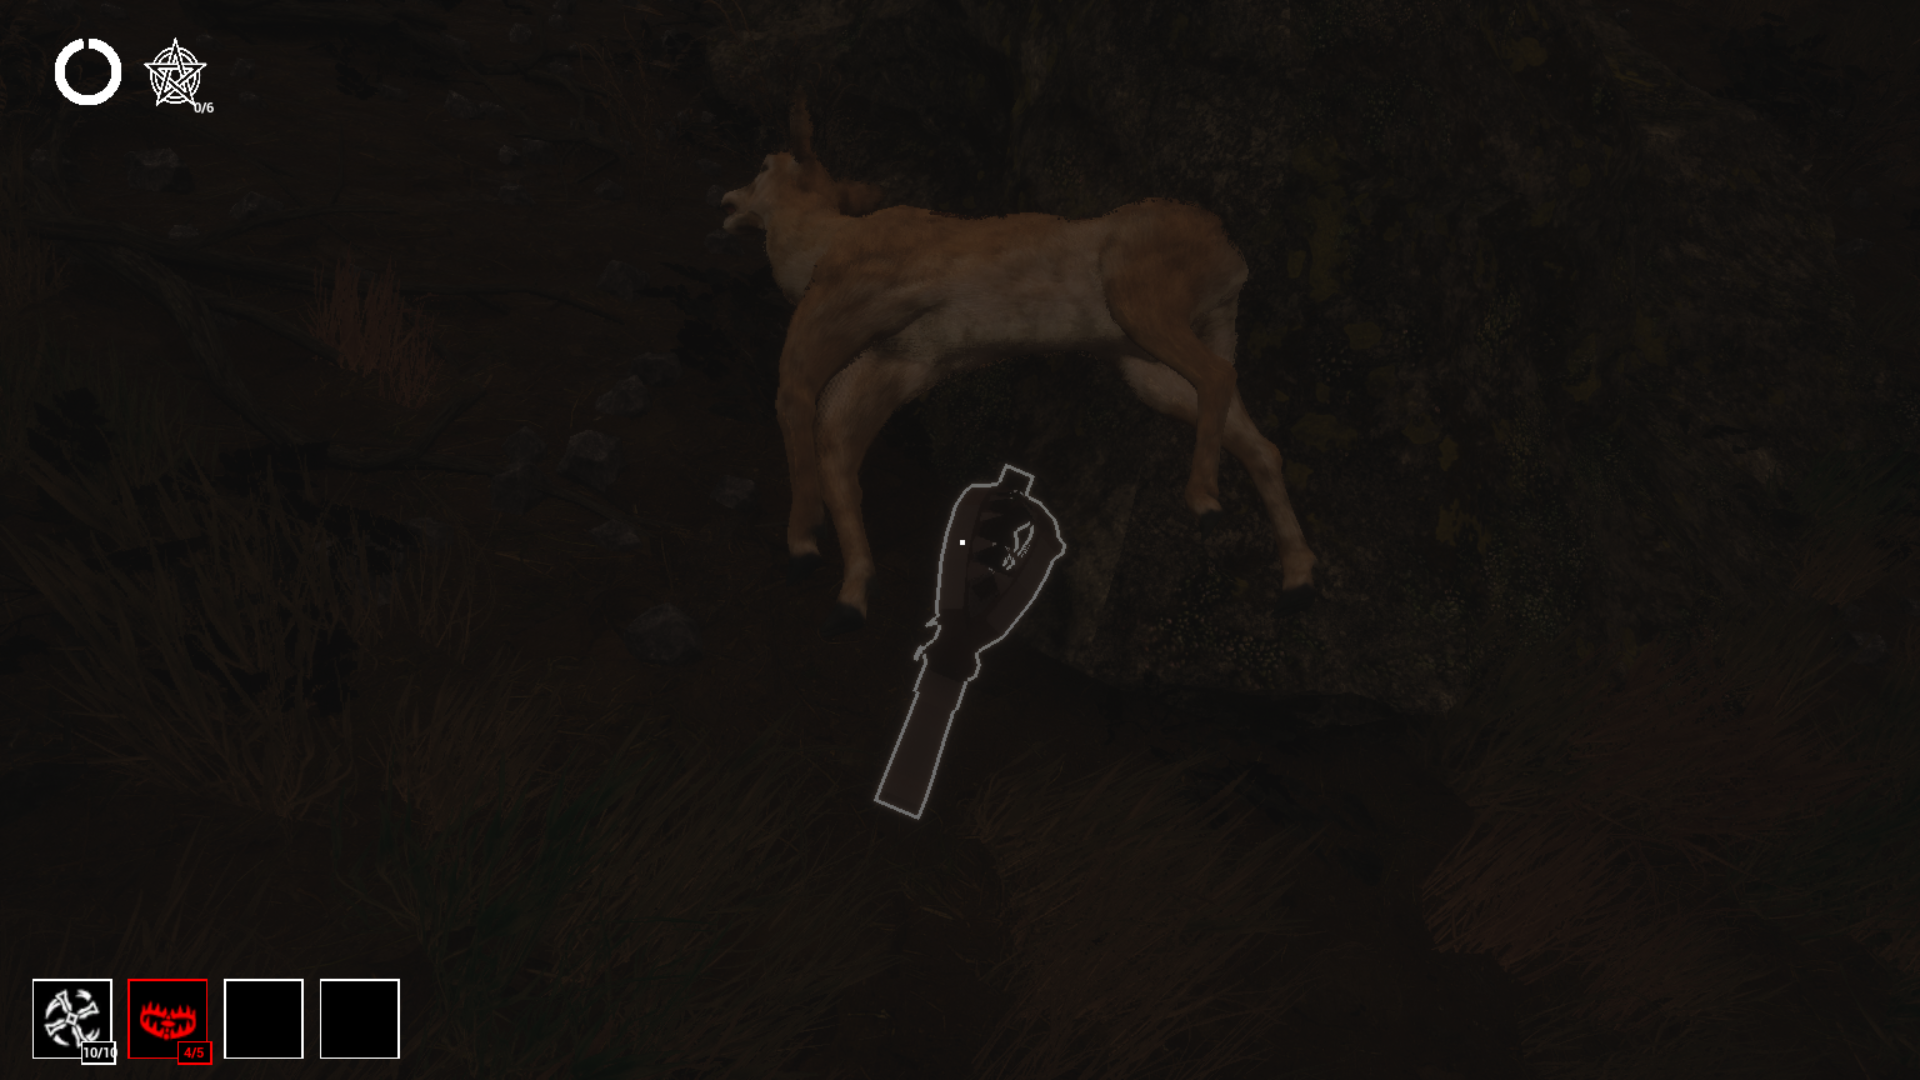
\includegraphics[width=\textwidth]{./img/mechanics/deer_trapped.png}
  \end{center}
    \caption[การจับกวางด้วยกับดัก]{การจับกวางด้วยกับดัก}
    \label{fig:trap}
\end{figure}

\begin{figure}[p]
  \begin{center}
  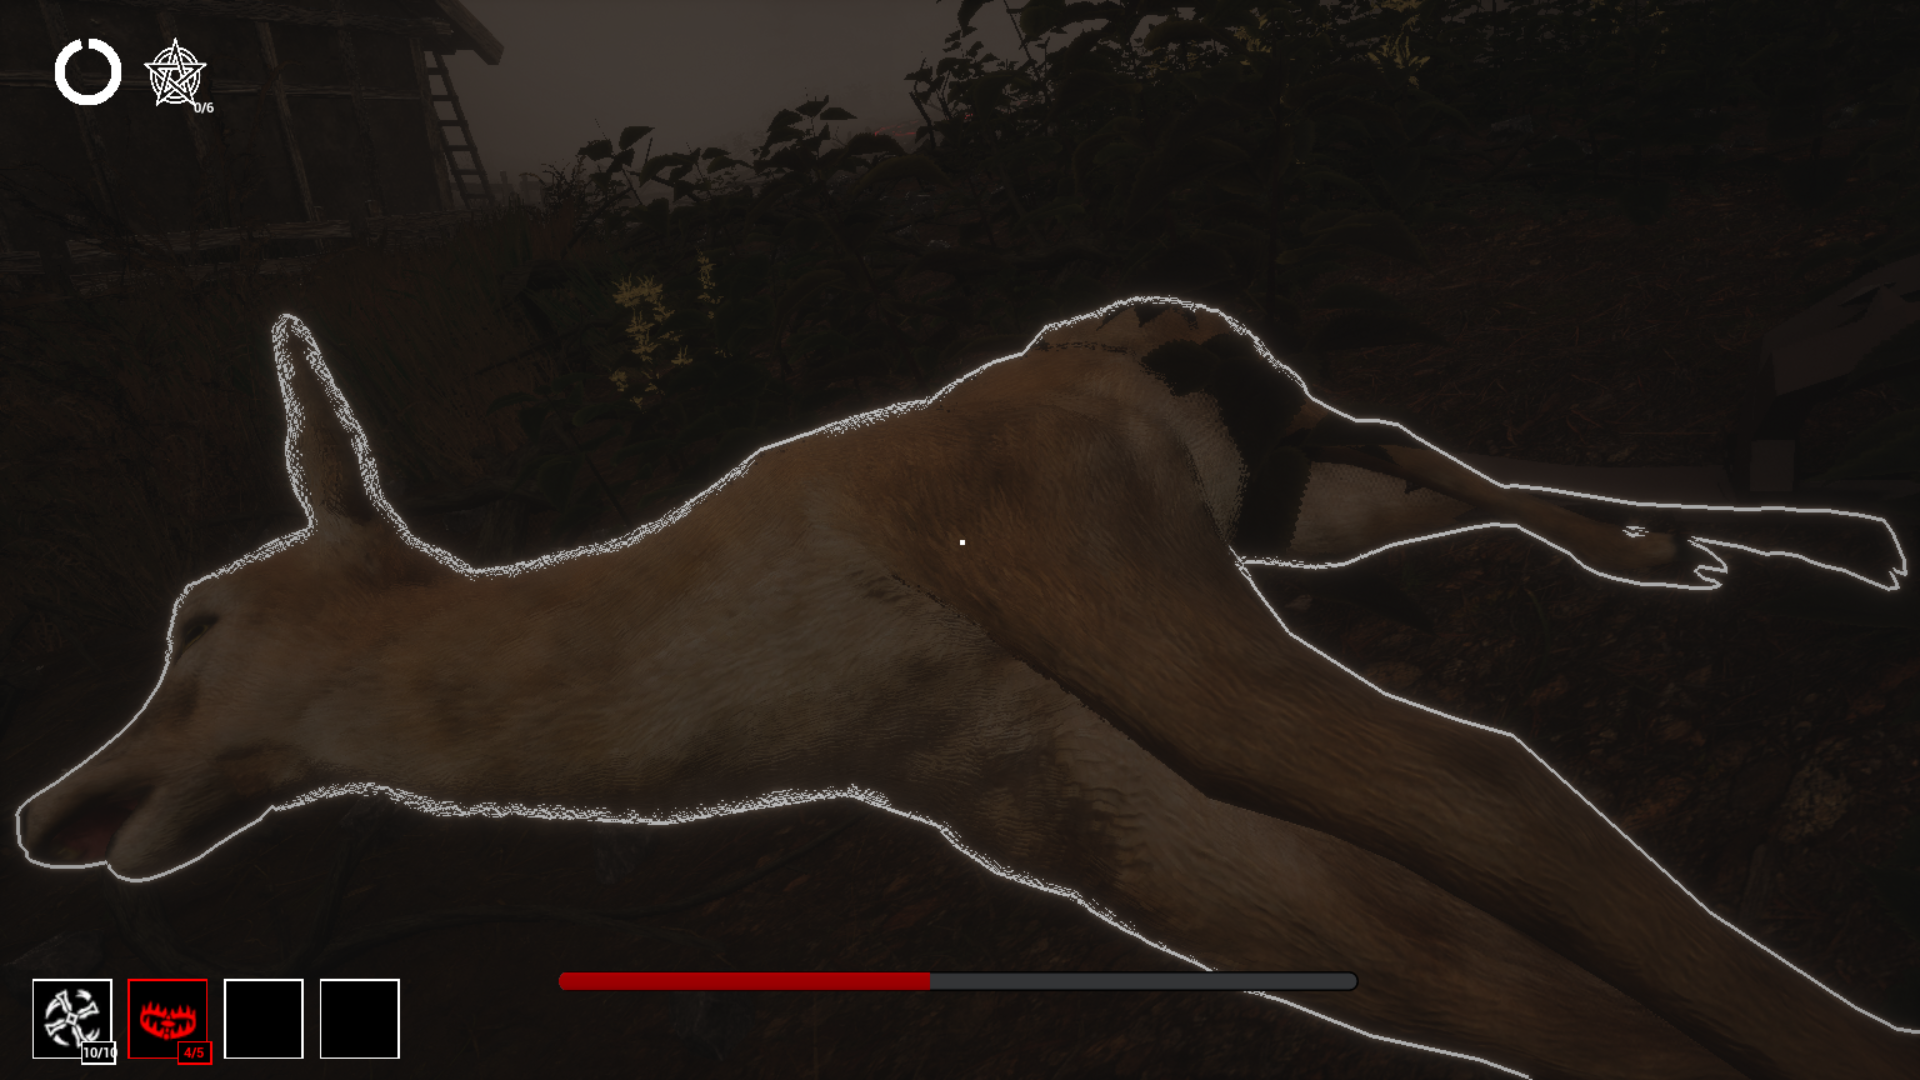
\includegraphics[width=\textwidth]{./img/mechanics/extract_blood.png}
  \end{center}
  \caption[การสกัดเลือดจากตัวกวาง]{การสกัดเลือดจากตัวกวาง}
  \label{fig:blood}
\end{figure}

\subsubsection{การทำพิธี}

เมื่อ Hunter ได้ทำการสกัดเลือดจากกวางแล้ว Hunter สามารถเลือกทำพิธีกรรม โดยการนำเลือดที่สกัดไปทำพิธีตามจุดที่กำหนดไว้จุดไหนก็ได้ ดังแสดงในรูปที่ ~\ref{fig:ritual}
ซึ่งจะมีกำหนดแบบสุ่มไว้ 3 จุด และสามารถทำซ้ำจุดเดิมได้ ซึ่งเมื่อผู้เล่นคนนั้นทำพิธีเสร็จสิ้นแล้ว 1 ครั้ง เขาจะได้รับการฟื้นฟู 
HP 1 ระดับ ในการทำพิธี 1 ครั้งจะใช้เวลา 30 วินาที สามารถยกเลิกการทำพิธีได้ แต่ต้องเริ่มทำพิธีใหม่ทั้งหมด

\begin{figure}[h]
  \begin{center}
  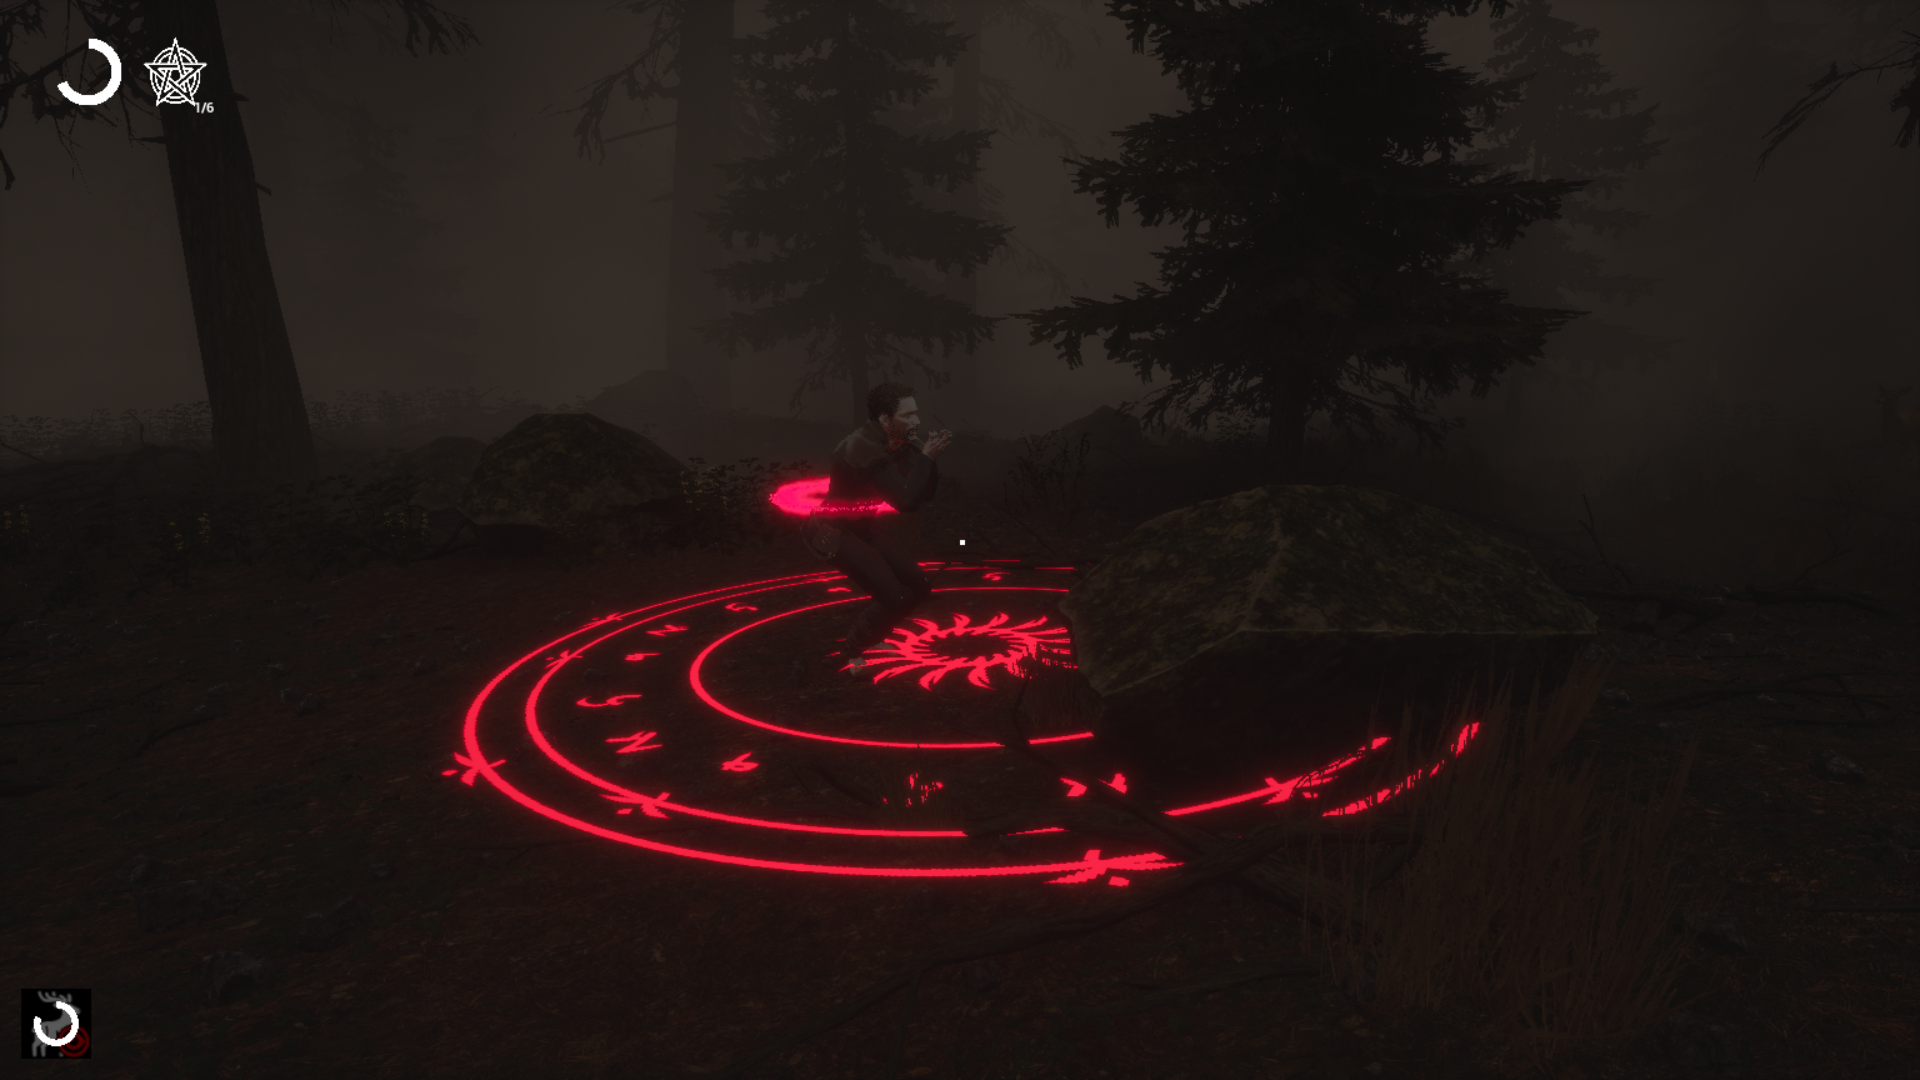
\includegraphics[width=\textwidth]{./img/mechanics/ritual-complete.png}
  \end{center}
  \caption[ภาพการทำพิธีของ Hunter จากมุมมองของผู้เล่นอีกคน]{ภาพการทำพิธีของ Hunter จากมุมมองของผู้เล่นอีกคน}
  \label{fig:ritual}
\end{figure}

\subsubsection{การโจมตี Witch}

Hunter สามารถโจมตี Witch ได้ด้วยการปามีดศักดิ์สิทธิ์ใส่ Witch หรือปักไว้ที่พื้นเพื่อล่อให้ Witch มาเหยียบ การโจมตี Witch นี้จะทำให้ Witch สะดุดและเดินช้าลง 
รวมถึงทำให้มองไม่เห็นชั่วครู่ ดังแสดงในรูปที่ \ref{fig:blind} ในระหว่างนี้ Hunter สามารถวิ่งไปแอบหลังต้นไม้หรือก้อนหิน เพื่อหลุดจากการไล่ล่าและทำพิธีต่อ

\begin{figure}[h]
  \begin{center}
  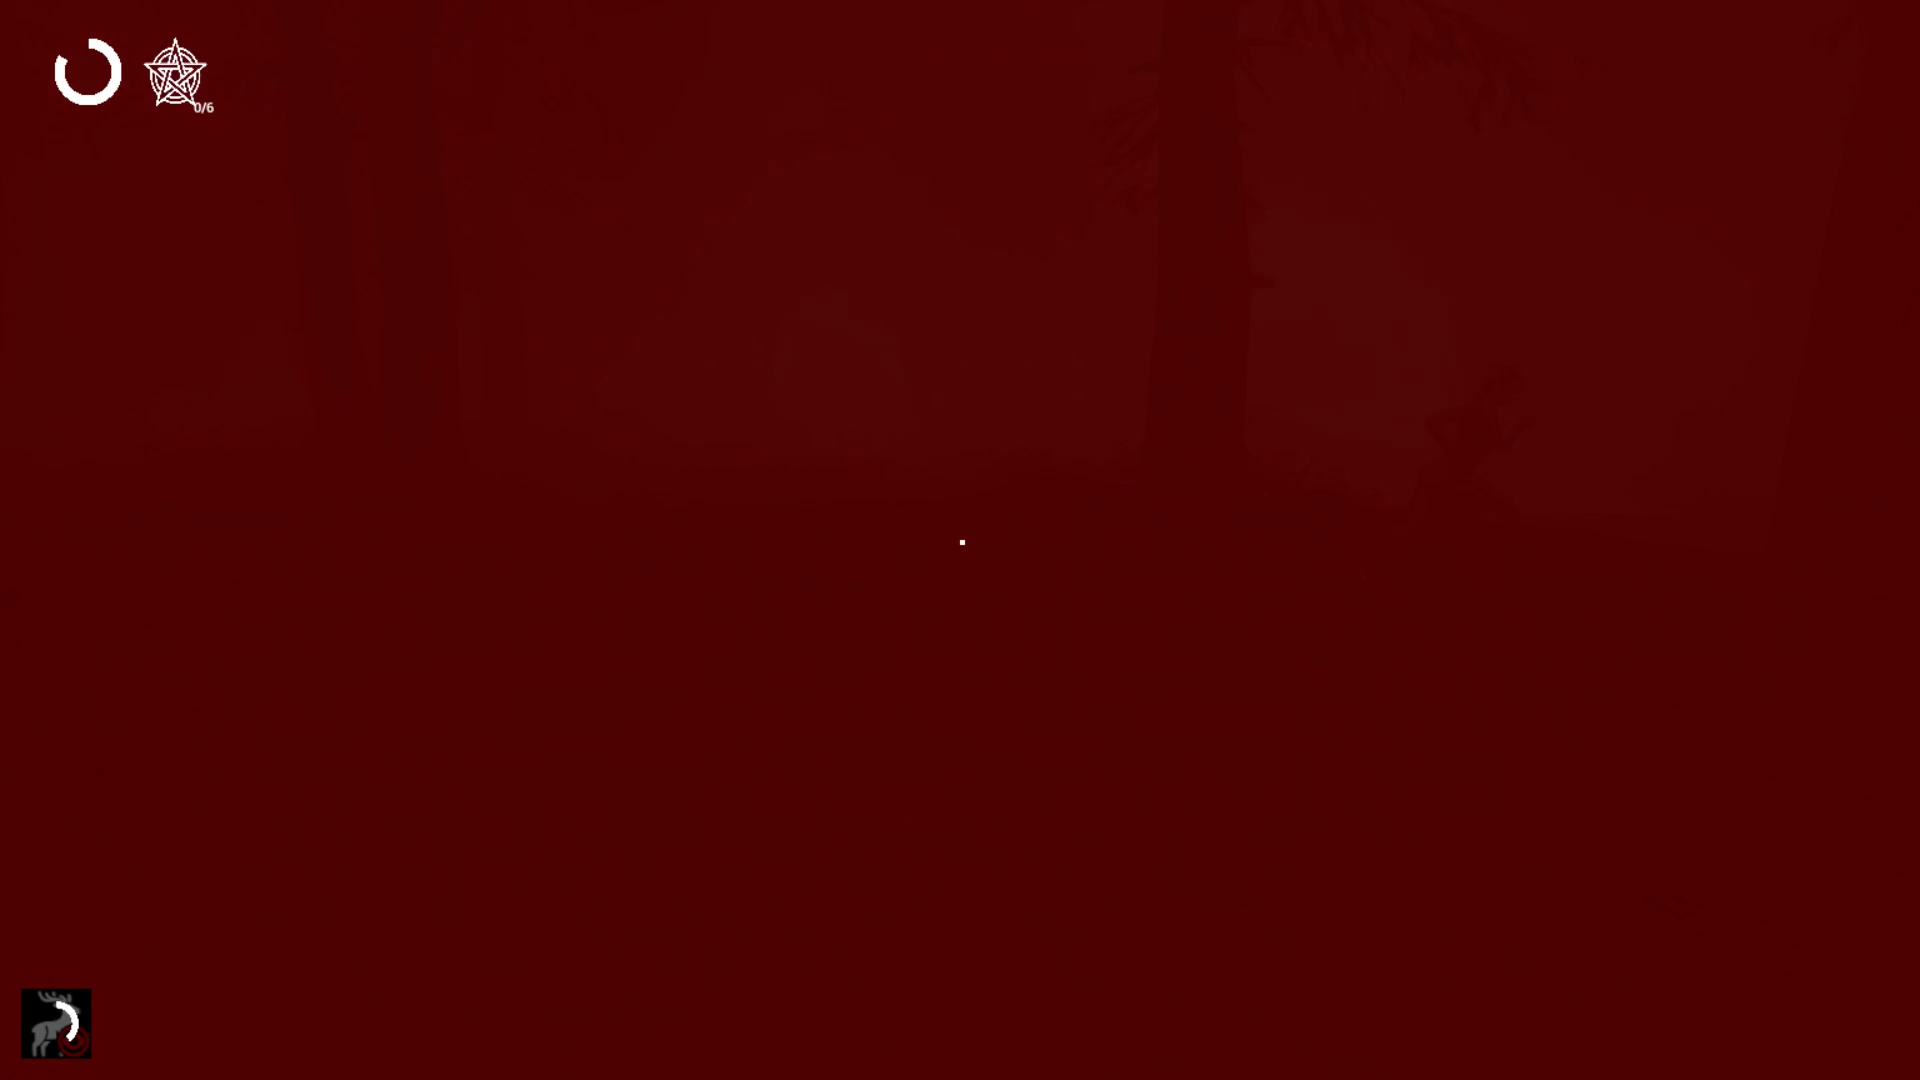
\includegraphics[width=\textwidth]{./img/mechanics/witch_blind.png}
  \end{center}
  \caption[Witch จะตาบอดและเดินไม่ได้ชั่วครู่เมื่อถูกโจมตี]{Witch จะตาบอดและเดินไม่ได้ชั่วครู่เมื่อถูกโจมตี}
  \label{fig:blind}
\end{figure}

\subsubsection{ระบบ Inventory}

Hunter สามารถเก็บ ใช้ และดร็อปไอเทมได้ ทำให้สามารถส่งต่อไอเทมให้ผู้เล่นอีกคนได้อีกด้วย Inventory มีทั้งหมด 4 ช่องตามรูปที่ ~\ref{fig:inventory} และไม่สามารถขยายได้เมื่อช่องเต็มแล้ว
โดยไอเทมที่สามารถเก็บและใช้ได้ มีดังนี้
\begin{enumerate}
  \item มีดศักดิ์สิทธิ์ มีให้ 10 เล่ม stack ได้ 10 เล่ม ปามีดแล้วสามารถเก็บมาใช้ซ้ำได้
  \item กับดักสัตว์ มีให้ 5 อัน stack ได้ 5 อัน กับดับสามารถวางไว้ได้ทุกที่ และสามารถเก็บมาใช้ซ้ำได้
  \item หลอดบรรจุเลือดของกวางที่ได้หลังจากการสกัดเลือด stack ได้ 3 หลอด
\end{enumerate}

\begin{figure}[h]
  \begin{center}
  
\includegraphics[width=0.5\textwidth]{./img/mechanics/inventory.png}
  \end{center}
  \caption[ระบบ Inventory]{ระบบ Inventory}
  \label{fig:inventory}
\end{figure}

\subsubsection{ระบบ HP}

HP ของ Hunter มี 3 ระดับ โดยเมื่อถูกโจมตีจาก Witch จะลดลง 1 ระดับ และสามารถฟื้นฟู HP 1 ระดับได้ด้วยการทำพิธี 
1 ครั้ง แต่ไม่สามารถฟื้นฟู HP จนมากกว่า 3 ระดับได้

ในเกมจะไม่แสดงหลอดเลือดแต่แสดงเป็น Vignette Effect สีแดงบนจอตามรูปที่ ~\ref{fig:damage_effect} ซึ่งจะรุนแแรงขึ้นเรื่อย ๆ ตามระดับ HP ที่ลดลงไป

\begin{figure}[p]
  \begin{center}
  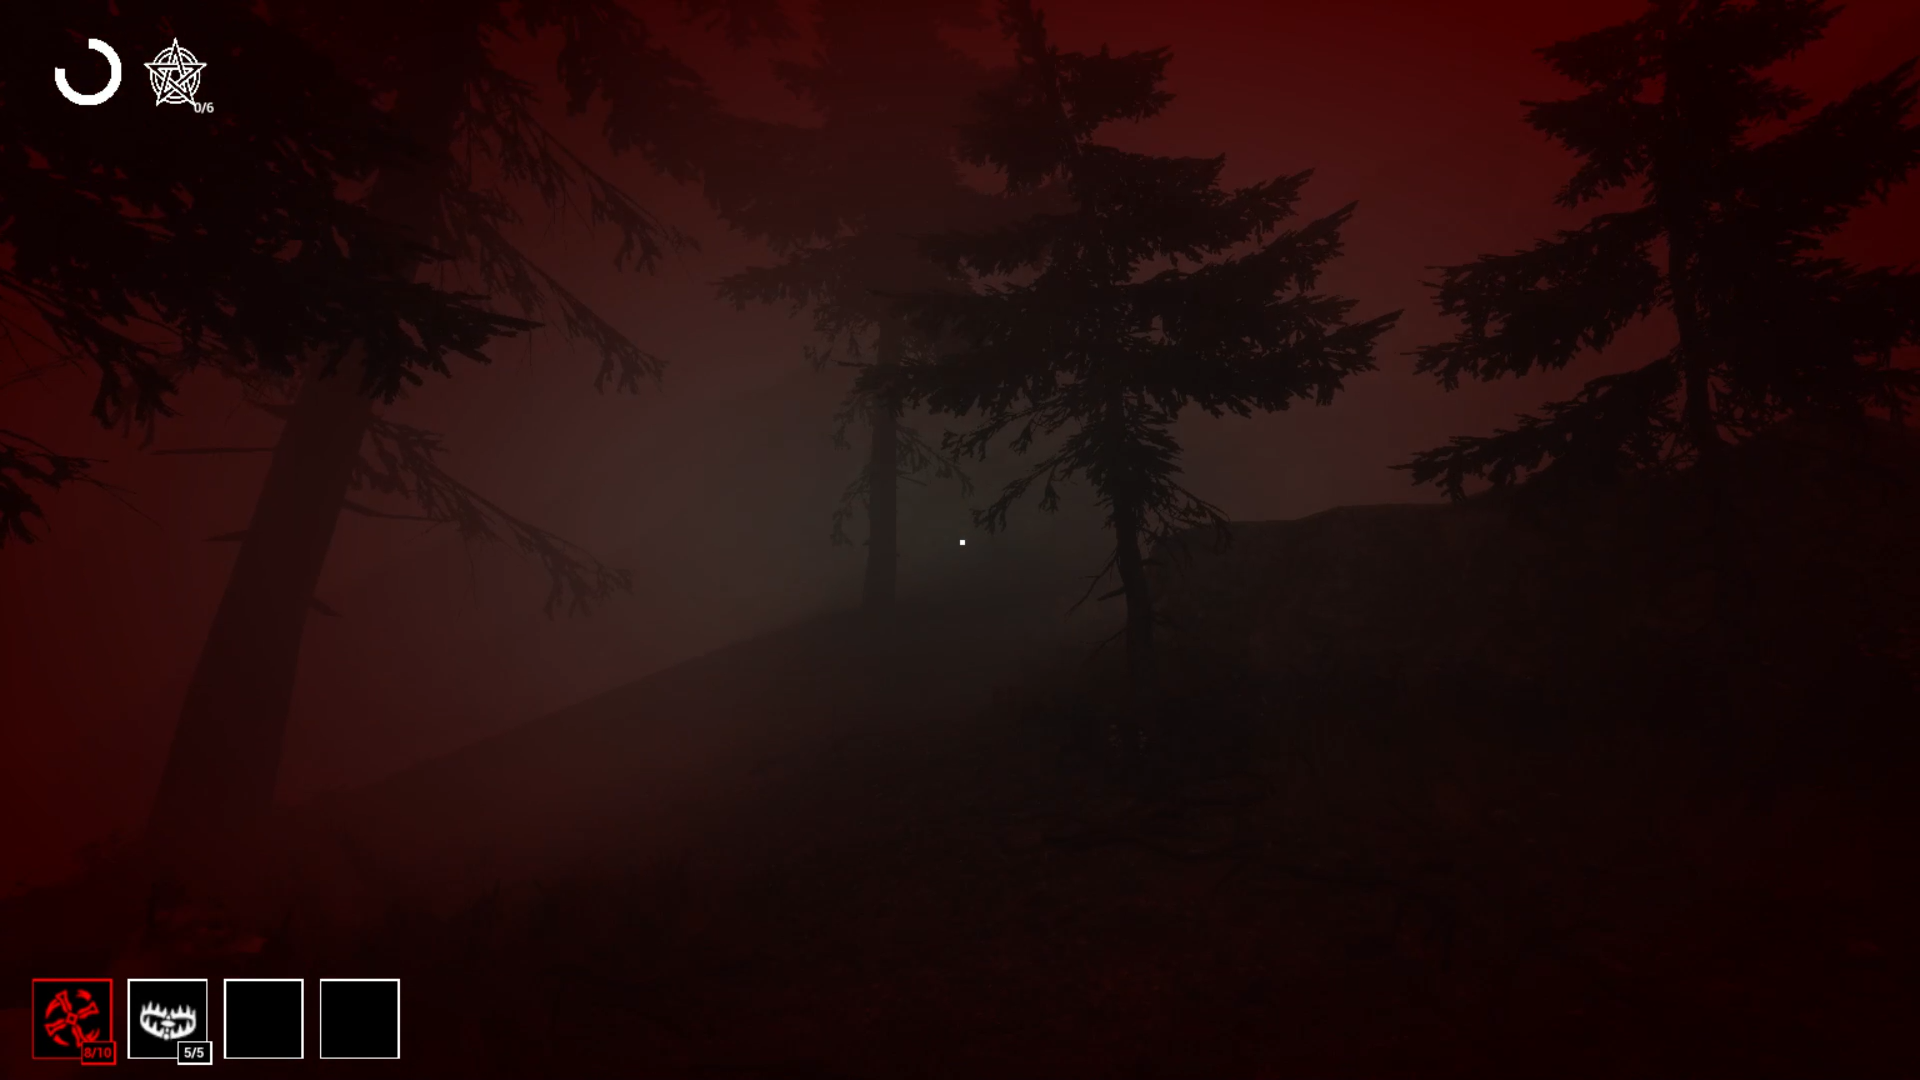
\includegraphics[width=\textwidth]{./img/mechanics/damage_effect.png}
  \end{center}
  \caption[Effect เมื่อ Hunter บาดเจ็บ]{Effect เมื่อ Hunter บาดเจ็บ}
  \label{fig:damage_effect}
\end{figure}

\subsubsection{ระบบชุบชีวิต}

เมื่อ Hunter ไม่เหลือ HP แล้ว จะเข้าสู่สถานะชุบชีวิต Hunter จะเกิดใหม่เป็นร่างวิญญาณ ณ ร่างของผู้เล่นอีกคน 
สามารถเลือกที่จะเกิดใหม่ด้วยการเดินกลับไปสิงร่างเดิม หรือเลือกที่จะไม่เกิดใหม่แต่เล่นเป็น Spectator ได้ ผู้เล่นคนอื่น ๆ 
จะไม่สามารถเห็น Hunter ในร่างวิญญาณนี้ Hunter แต่ละคนสามารถชุบชีวิตได้เพียง 1 ครั้งเท่านั้น มุมมองของผู้เล่นที่เป็นร่างวิญญาณ แสดงในรูปที่ ~\ref{fig:revive}

\begin{figure}[p]
  \begin{center}
  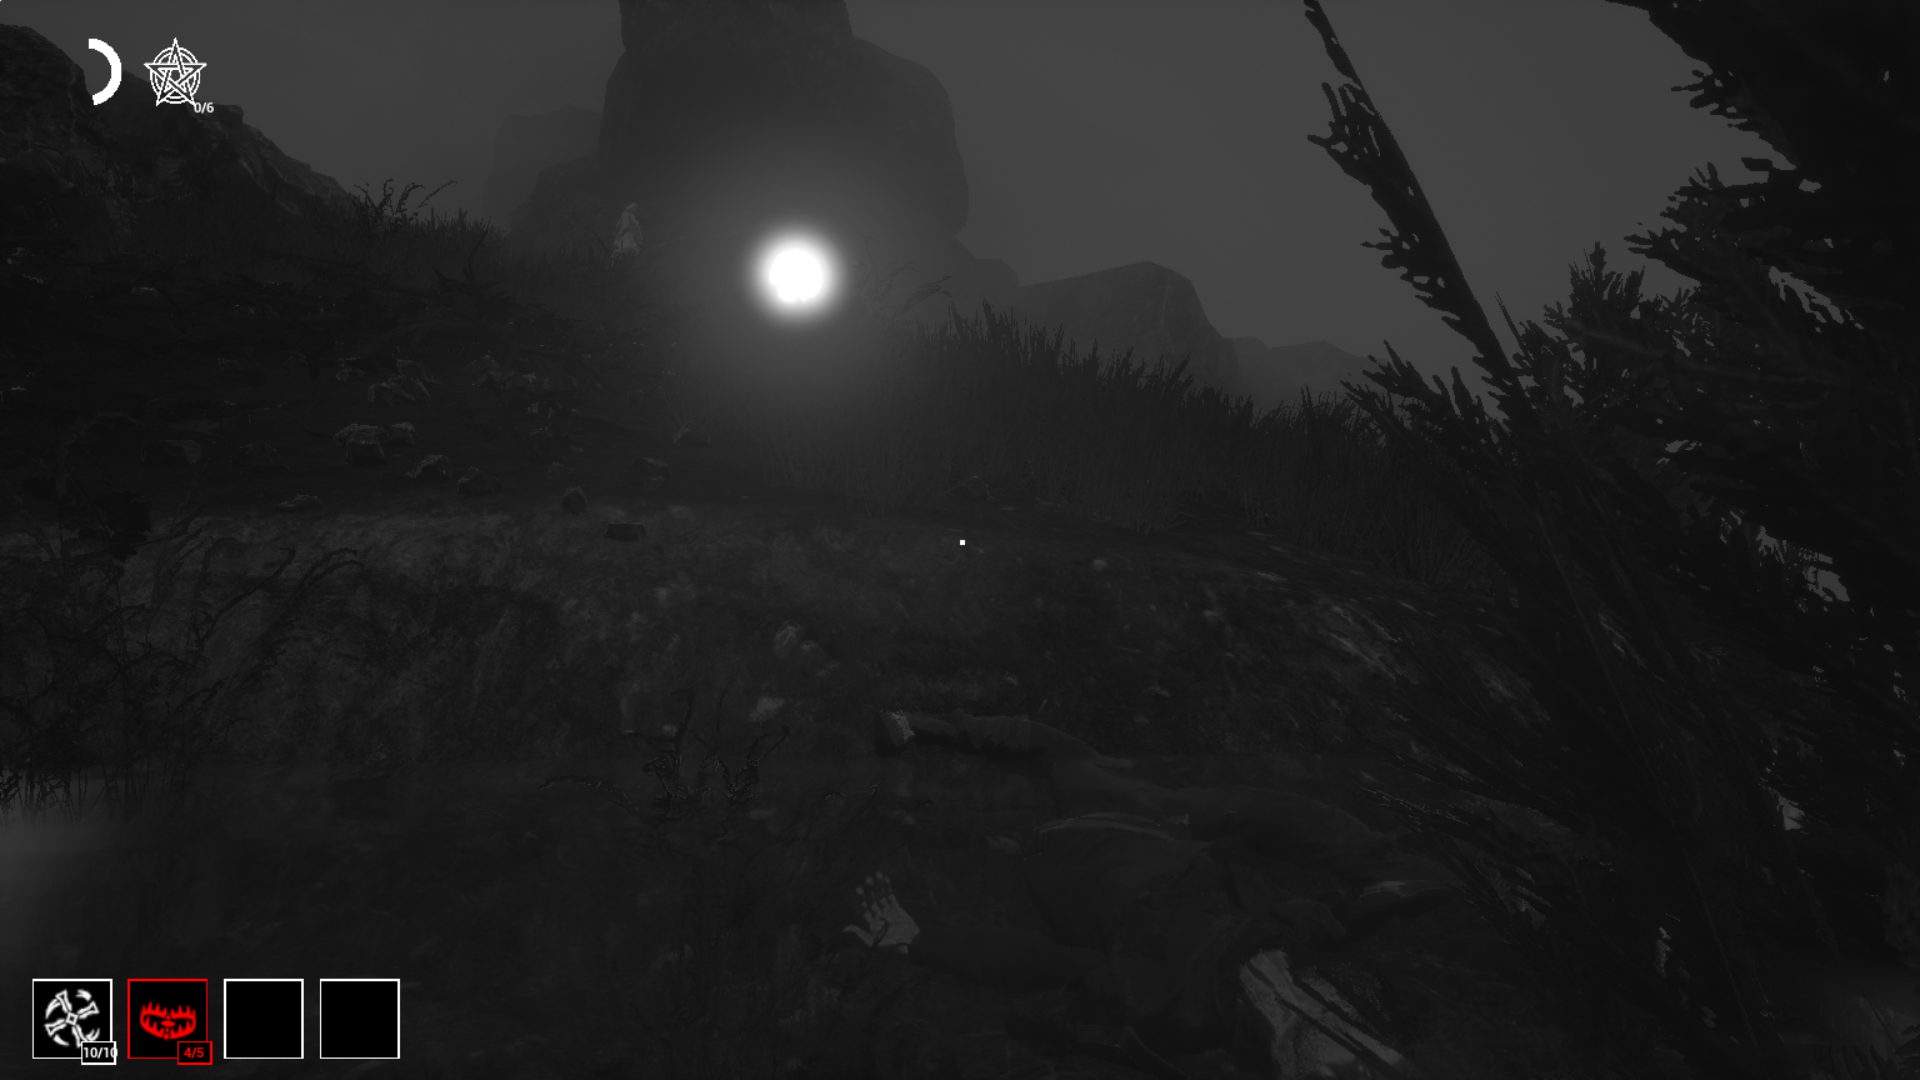
\includegraphics[width=\textwidth]{./img/mechanics/revive.png}
  \end{center}
  \caption[ภาพแสดงมุมมองของผู้เล่นที่เป็นร่างวิญญาณ ต้องสิงกลับร่างเดิมเพื่อชุบชีวิต]{ภาพแสดงมุมมองของผู้เล่นที่เป็นร่างวิญญาณ ต้องสิงกลับร่างเดิมเพื่อชุบชีวิต}
  \label{fig:revive}
\end{figure}

\subsection{การเล่นของฝ่าย Witch}

\subsubsection{การโจมตี Hunter}

Witch สามารถโจมตี Hunter ได้โดยการใช้เวทมนต์ 2 แบบ แบบระยะใกล้และระยะไกล โดยเมื่อโจมตีแล้ว 
Hunter จะลด HP ลง 1 ระดับ

\begin{enumerate}
  \item การโจมตีระยะใกล้ด้วยไอพิษ (Breath of Death): สามารถโจมตีได้ในระยะ 1-2 เมตร การโจมตีเป็นรูปแบบของการพ่นไอพิษ ดังแสดงในรูปที่ ~\ref{fig:short_range_attack}
  \item การโจมตีระยะไกลด้วยลูกไฟ (Inferno Soul): สามารถโจมตีในระยะไกลเท่าไหร่ก็ได้ การโจมตีเป็นรูปแบบของการยิงเวทมนต์ไฟ ดังแสดงในรูปที่ ~\ref{fig:long_range_attack}
(Fire Ball) โดยจะต้องมีการชาร์จพลังให้เต็มก่อนที่จะโจมตีในทุกครั้ง
\end{enumerate}

\begin{figure}[p]
  \begin{center}
  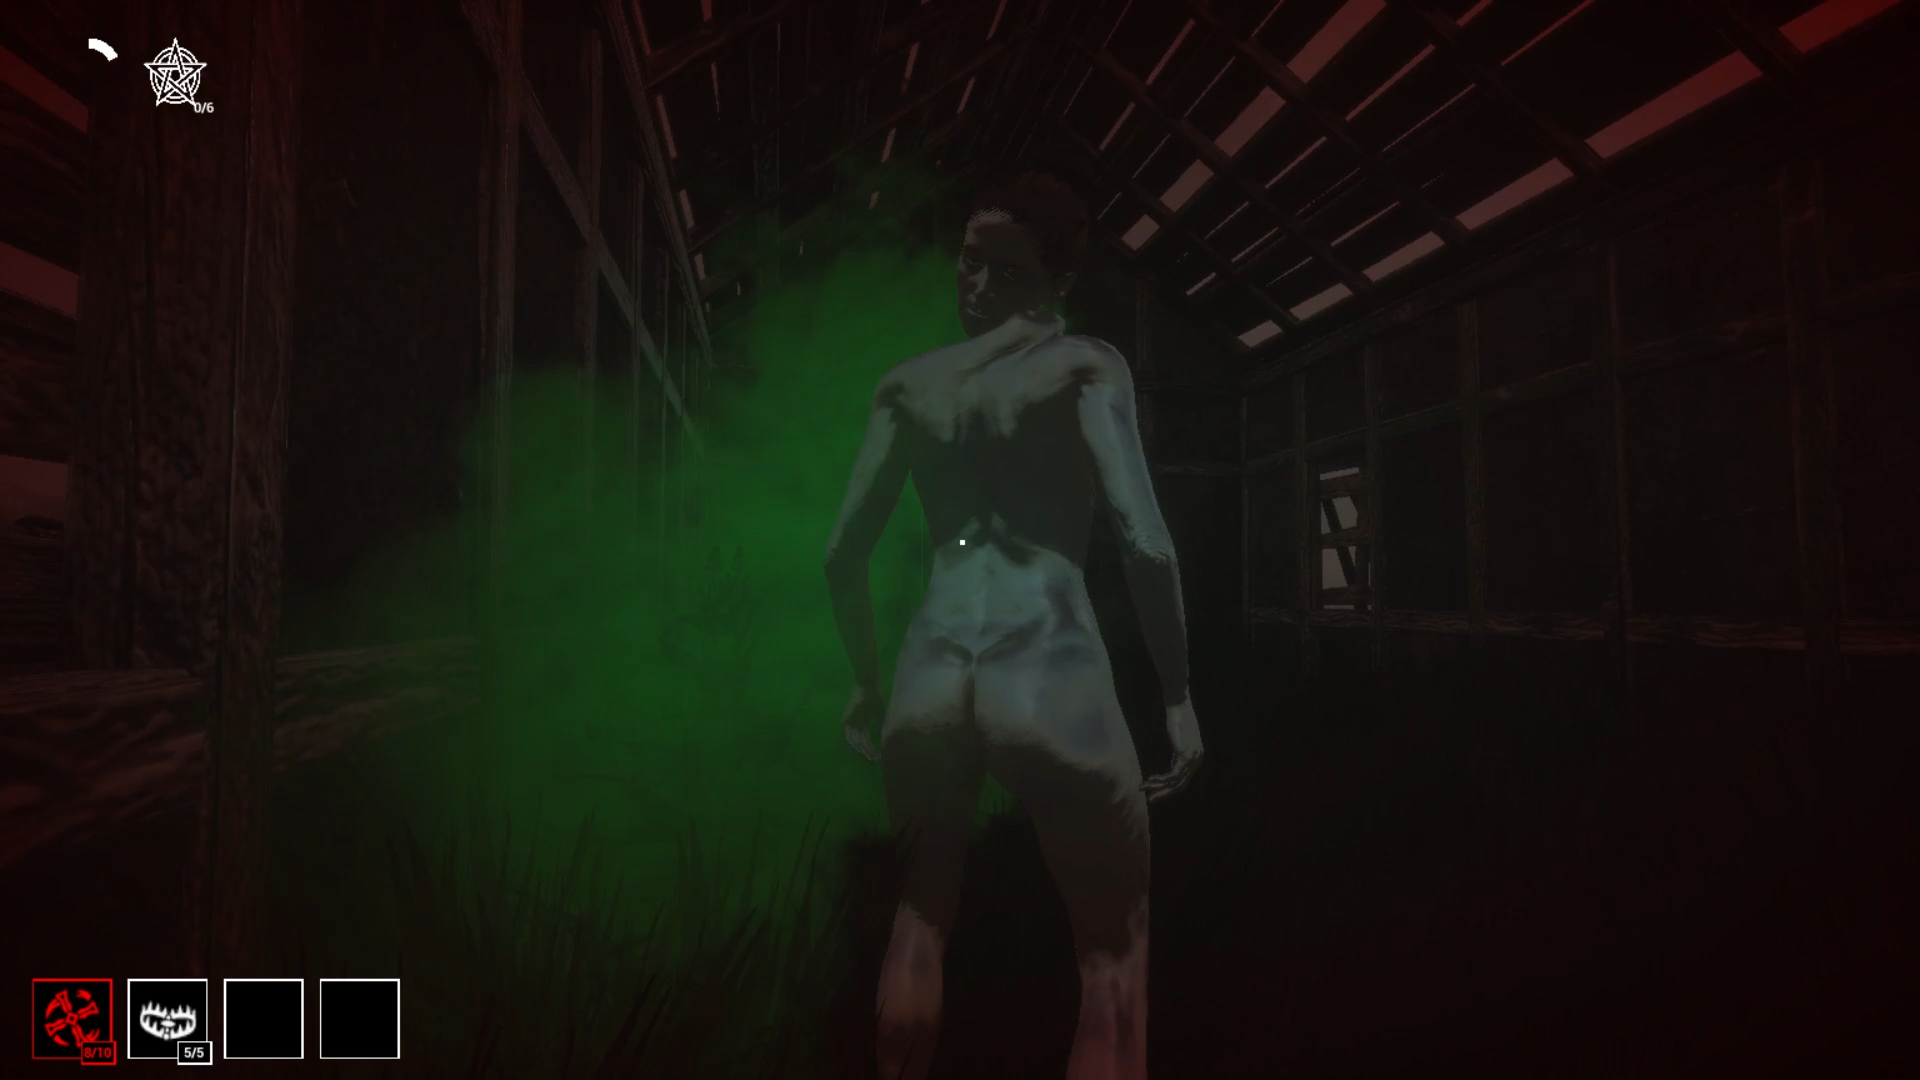
\includegraphics[width=\textwidth]{./img/mechanics/breath_of_death.png}
  \end{center}
    \caption[การโจมตีระยะใกล้ด้วยไอพิษของ Witch]{การโจมตีระยะใกล้ด้วยไอพิษของ Witch}
    \label{fig:short_range_attack}    
\end{figure}

\begin{figure}[p]
  \begin{center}
  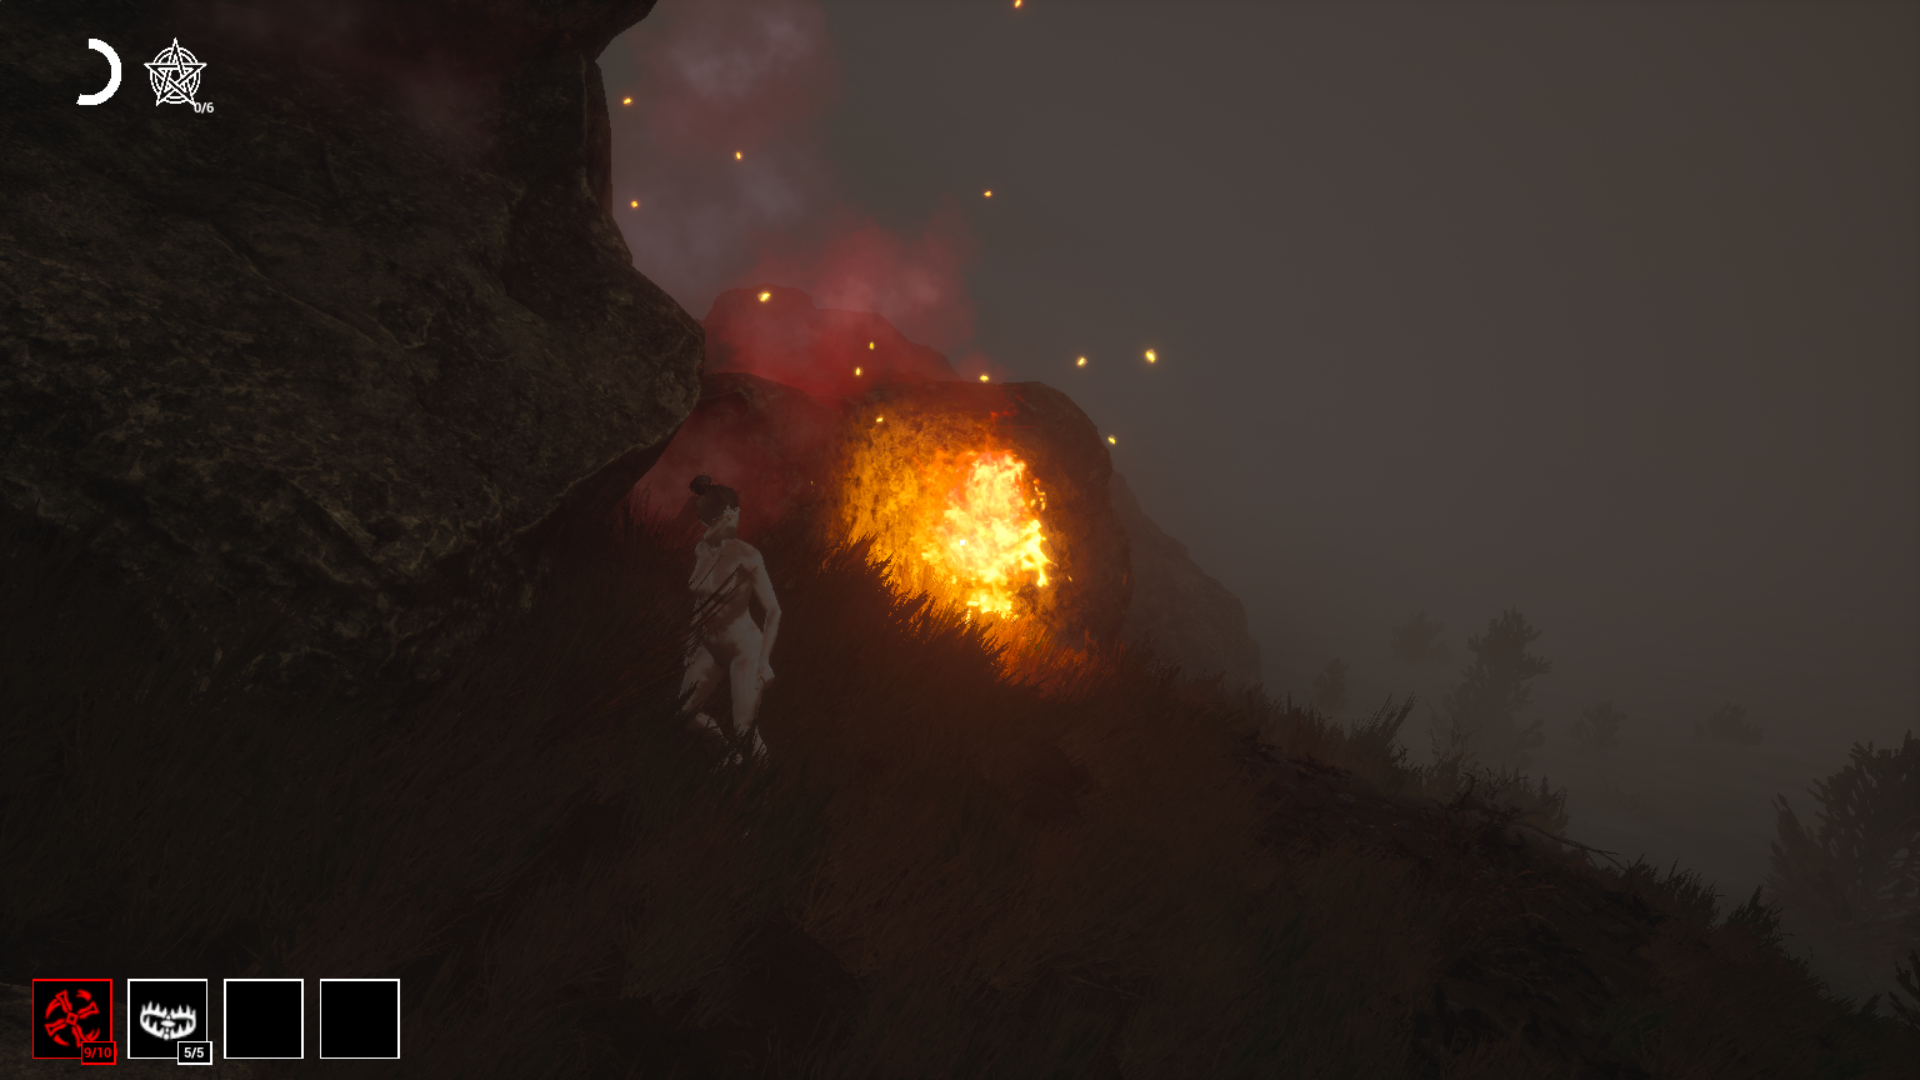
\includegraphics[width=\textwidth]{./img/mechanics/inferno_soul.png}
  \end{center}
    \caption[การโจมตีระยะไกลด้วยลูกไฟของ Witch]{การโจมตีระยะไกลด้วยลูกไฟของ Witch}\label{การโจมตีระยะไกลด้วยลูกไฟ}
    \label{fig:long_range_attack}
\end{figure}

\subsubsection{การเคลื่อนย้ายร่างไปเป็นกวาง}

Witch สามารถกดดูตำแหน่งและการเคลื่อนที่ของกวางในแมพได้ (Deer Vision) ดังแสดงในรูปที่ ~\ref{fig:deer_vision} ซึ่งสามารถใช้เลือกกวางที่จะย้ายร่างไปสิงได้
ความสามารถนี้สามารถใช้ได้ทุก ๆ 60 วินาที ในขณะเป็นกวางอยู่ ผู้เล่นไม่สามารถทำการโจมตีอีกฝั่งได้
ต้องกลับมาเป็นร่าง Witch เดิมก่อนทำการโจมตี ถ้าหากกวางที่ผู้เล่นสิงอยู่ถูกโจมตีจะทำให้วิญญาณกลับมาเป็นร่างเดิมทันที

\begin{figure}[p]
  \begin{center}
  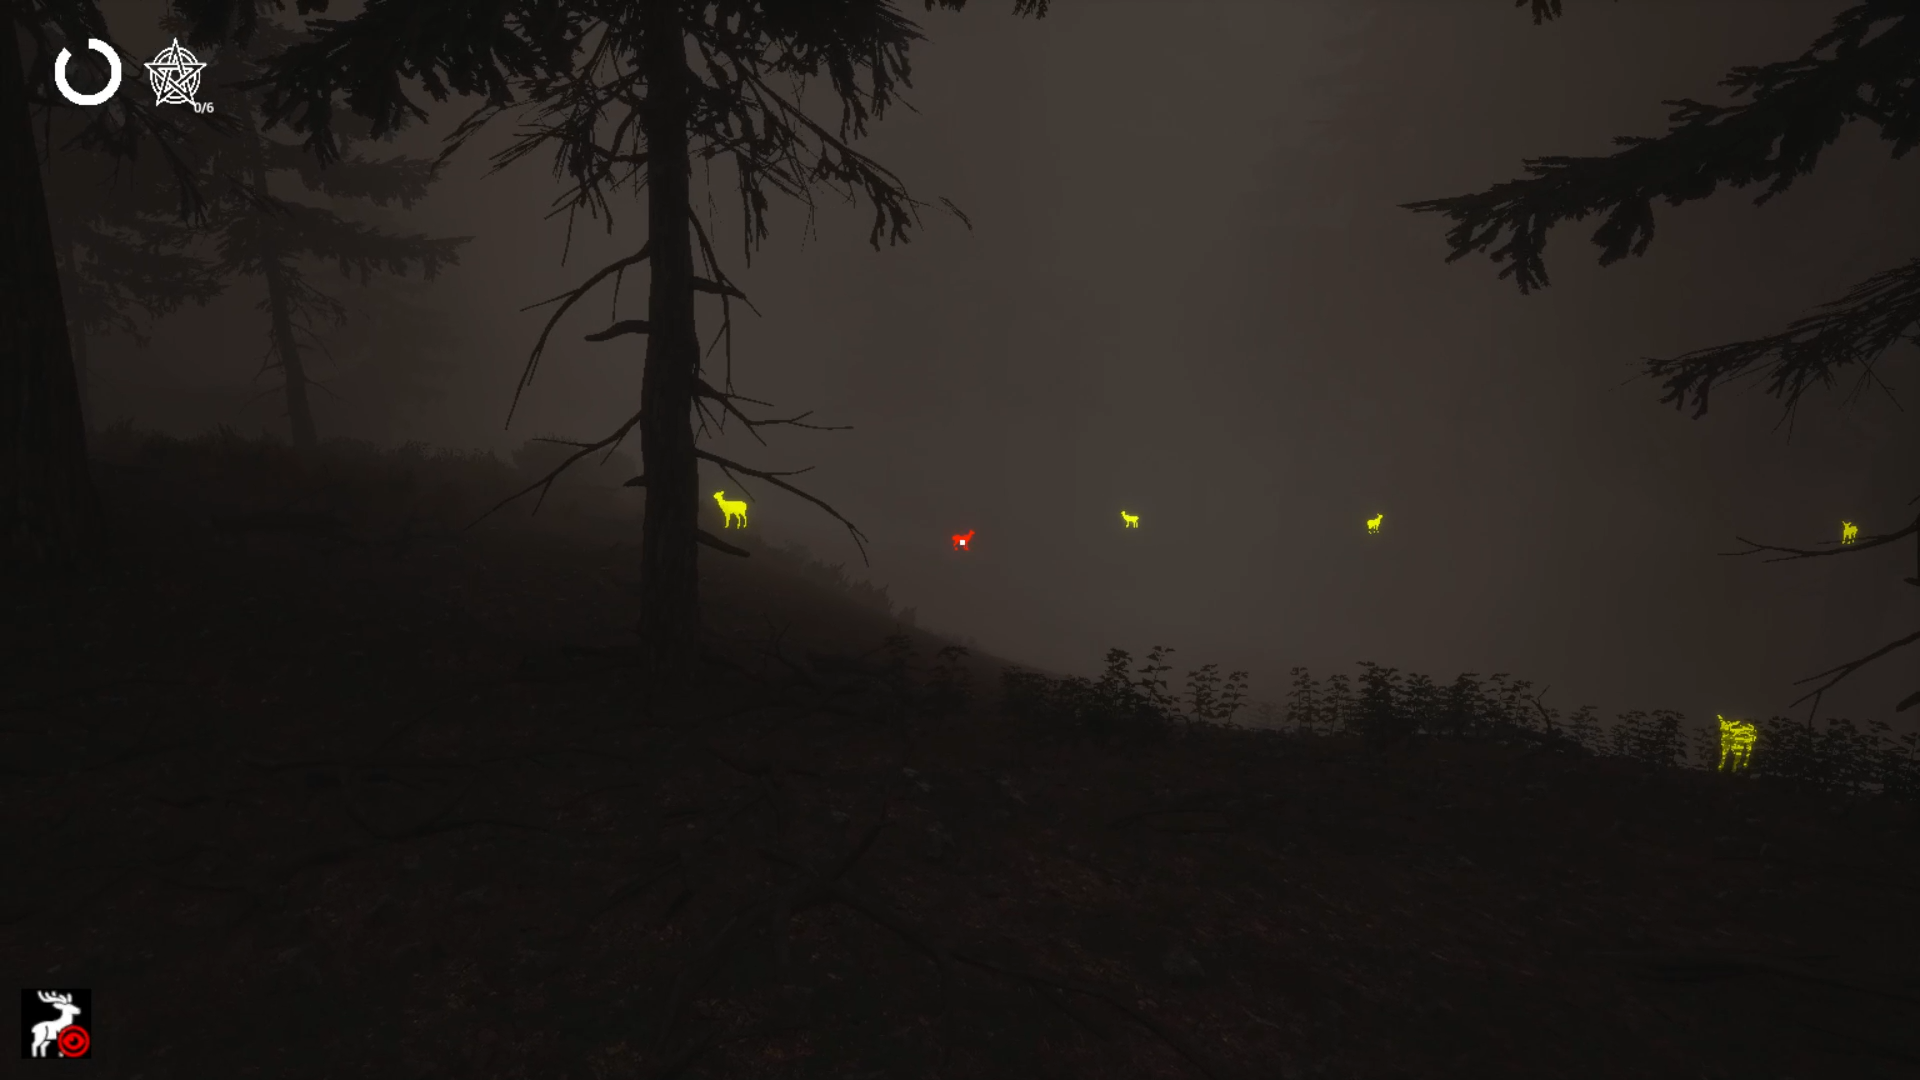
\includegraphics[width=\textwidth]{./img/mechanics/deervision.png}
  \end{center}
    \caption[Witch ใช้ความสามารถดูตำแหน่งของกวางที่สามารถสิงร่างได้ (Deer Vision)]{Witch ใช้ความสามารถดูตำแหน่งของกวางที่สามารถสิงร่างได้ (Deer Vision)}
    \label{fig:deer_vision}
\end{figure}

\begin{figure}[p]
  \begin{center}
  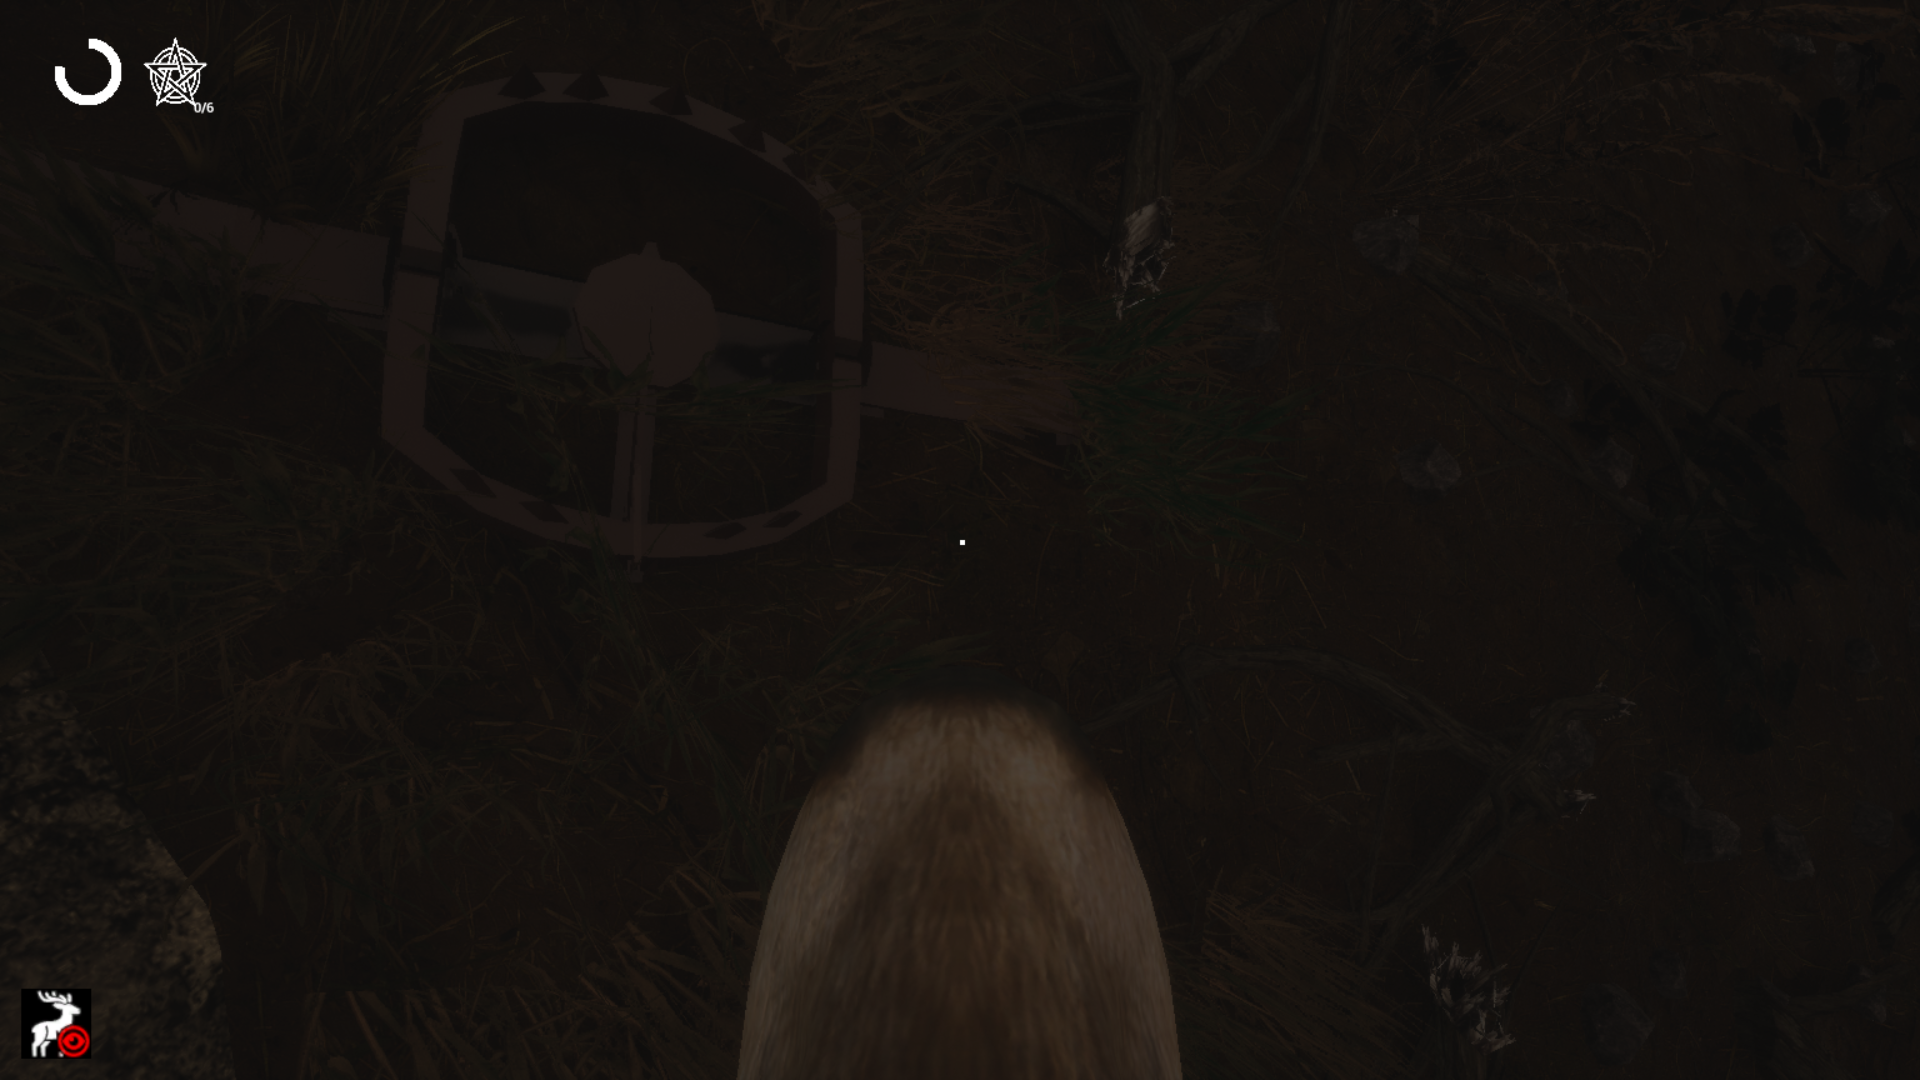
\includegraphics[width=\textwidth]{./img/mechanics/witch_deer.png}
  \end{center}
    \caption[มุมมองบุคคลที่หนึ่งของ Witch ที่เล่นเป็นกวาง]{มุมมองบุคคลที่หนึ่งของ Witch ที่เล่นเป็นกวาง}
    \label{fig:deer_view}
\end{figure}

\subsubsection{ความสามารถพิเศษอื่น ๆ}

\begin{itemize}
  \item สามารถมองเห็นตำแหน่งของจุดทำพิธีตอนเริ่มเกมได้ ดังแสดงในรูปที่ ~\ref{fig:see_ritual}
  \item สามารถได้ยินเสียงจุดทำพิธีและการทำพิธีได้ในระยะที่ค่อนข้างไกล
\end{itemize}

\begin{figure}[h]
  \begin{center}
  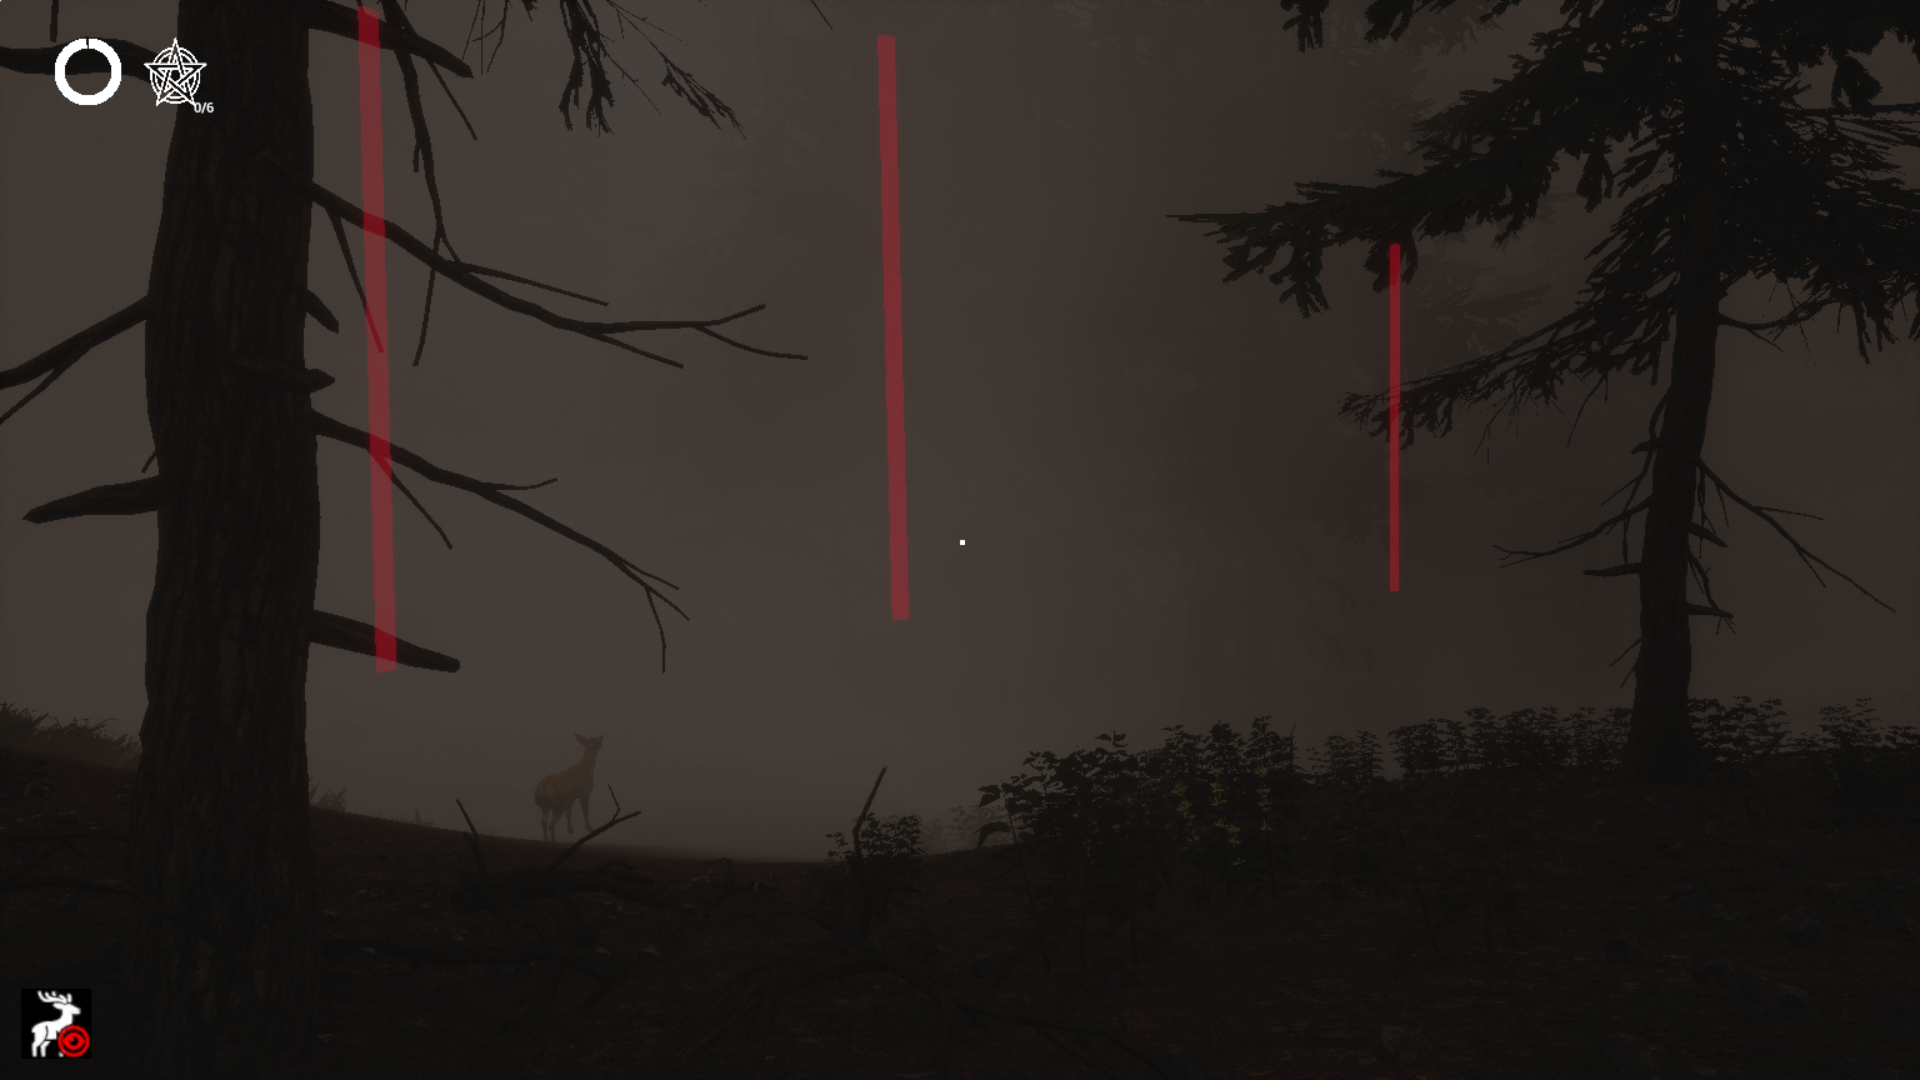
\includegraphics[width=\textwidth]{./img/mechanics/see_ritual.png}
  \end{center}
  \caption[Witch สามารถมองเห็นตำแหน่งของจุดทำพิธีตอนเริ่มเกมได้]{Witch สามารถมองเห็นตำแหน่งของจุดทำพิธีตอนเริ่มเกมได้}
  \label{fig:see_ritual}
\end{figure}

\subsection{เงื่อนไขการจบเกม}

\subsubsection{ฝ่าย Hunters ชนะ}

ฝ่าย Hunters ชนะเมื่อทำพิธีได้ครบ 6 ครั้ง ภายในเวลาที่กำหนดไว้

\subsubsection{ฝ่าย Witch ชนะ} 

ฝ่าย Witch ชนะเมื่อ Hunter ทุกคนไม่สามารถชุบร่างใหม่ได้แล้วหรือ Hunter ทุกคนเสียชีวิตกลายเป็นร่างวิญญาณทั้งหมดพร้อมกัน 
หรือฝ่าย Hunters ไม่สามารถทำพิธีได้ครบ 6 ครั้งภายในเวลาที่กำหนดไว้

\pagebreak

\section{การออกแบบระบบ}

เกมนี้ถูกพัฒนาโดยใช้ Unreal Engine version 5.1.1 เพื่อให้ได้ภาพและบรรยากาศที่สวยงามและสมจริง
อีกทั้ง Game Engine นี้ยังรองรับการพัฒนาเกมแบบ Multiplayer ได้ดี และมีเครื่องมือที่สามารถช่วยในการพัฒนา

\subsection{การออกแบบระบบ Multiplayer}

เกมนี้ถูกออกแบบให้เล่นแบบ Multiplayer โดยมีการเชื่อมต่อผ่าน Local Area Network (LAN) เท่านั้น
โดยจะมี 1 ผู้เล่นเป็น Host ทำหน้าที่เป็นทั้ง Server และ Client เรียกว่า Listen Server
\begin{itemize}
  \item Server มีหน้าที่เป็นตัวกลางในการเชื่อมต่อระหว่างผู้เล่นทั้งหมด ควบคุมการเกิดเหตุการณ์ในเกมและ Logic ที่สำคัญต่อการเล่น
  \item Client เป็นผู้เล่นที่เชื่อมต่อเข้ามาเล่นเกมและต้องส่งข้อมูลการกระทำของผู้เล่นไปยัง Server เช่น Input การโจมตี การเคลื่อนที่ 
  ซึ่ง Server จะทำการตรวจสอบความถูกต้องและส่งต่อการแสดงผล เช่น Effect การโจมตี การเคลื่อนที่ กลับไปยัง Client ที่เกี่ยวข้อง
\end{itemize}

การเชื่อมต่อระหว่าง Server และ Client ใช้โปรโตคอล UDP ซึ่งเป็นโปรโตคอลที่เหมาะสำหรับการเชื่อมต่อแบบ Real-time ที่จะต้องมีการส่งข้อมูลไปมาอย่างรวดเร็ว
เช่น ในเกม Multiplayer ที่ต้องการให้ผู้เล่นสามารถเคลื่อนที่ โจมตี หรือทำการกระทำอื่น ๆ ได้ทันที อีกทั้งยังต้องทำให้ผู้เล่นสามารถเห็นผลลัพธ์ทันทีโดยไม่ขาดหาย
โดยเฉพาะสิ่งที่ส่งผลต่อการเล่น เช่น การทำพิธี การตายของผู้เล่น การชุบชีวิต

\subsection{การออกแบบโปรแกรมส่วนระบบการเล่น}

ผู้พัฒนาได้เลือกใช้ Blueprint ซึ่งคือ Visual Scripting ที่ใช้ในการพัฒนาเกมด้วย Unreal Engine 
Visual Scripting สามารถทำให้ผู้พัฒนาสามารถพัฒนาเกมได้ไวขึ้น และทำให้ผู้พัฒนาสามารถทำงานร่วมกันได้ง่ายขึ้น
ทั้ง 2 ฝั่งมีความสามารถที่แตกต่างกัน ทางผู้พัตนาจึงได้เลือกใช้ Blueprint Actor Component สำหรับโค้ดส่วนที่เป็นความสามารถพิเศษของแต่ละฝั่ง
Blueprint Actor Component คือโมดูลที่สามารถเพิ่มเข้าไปใน Actor หรือตัวละครได้ โมดูลหนึ่งโมดูลจะประกอบไปด้วยโค้ดที่เป็นส่วนที่เกี่ยวข้องกับความสามารถใด 
ความสามารถหนึ่งเท่านั้นตามที่กล่าวไปในวิธีการเล่น ทำให้โค้ดของระบบการเล่นมี Modularity มากขึ้น เกิด Encapsulation และ Separation of Concerns ระหว่างแต่ละความสามารถ

\subsection{การออกแบบ User Interface}

User Interface (UI) ของเกมถูกออกแบบโดยใช้ UMG (Unreal Motion Graphics) ซึ่งเป็นเครื่องมือที่ใช้ในการออกแบบ UI ของเกมใน Unreal Engine
UMG ประกอบไปด้วย Widget ต่าง ๆ ที่ผู้พัฒนาสามารถลากวางและแก้ไขบนหน้าจอ และสามารถเขียนโค้ดโดยใช้ Blueprint เพื่อควบคุมการทำงานของ Widget ได้

UI ของเกมเป็นแบบเรียบง่าย จะแสดงเพียงสิ่งที่จำเป็นเท่านั้น UI บางส่วนจะแสดงขึ้นเมื่อผู้เล่นปฏิสัมพันธ์กับสิ่งของในเกมหรือทำความสามารถพิเศษเท่านั้น 
เพื่อให้ผู้เล่นได้ดื่มด่ำกับบรรยากาศเปรียบเสมือนเล่นเป็นตัวละครนั้นจริง ๆ

\subsubsection{UI ขณะเริ่มเกม}

\begin{figure}[h]
  \begin{center}
  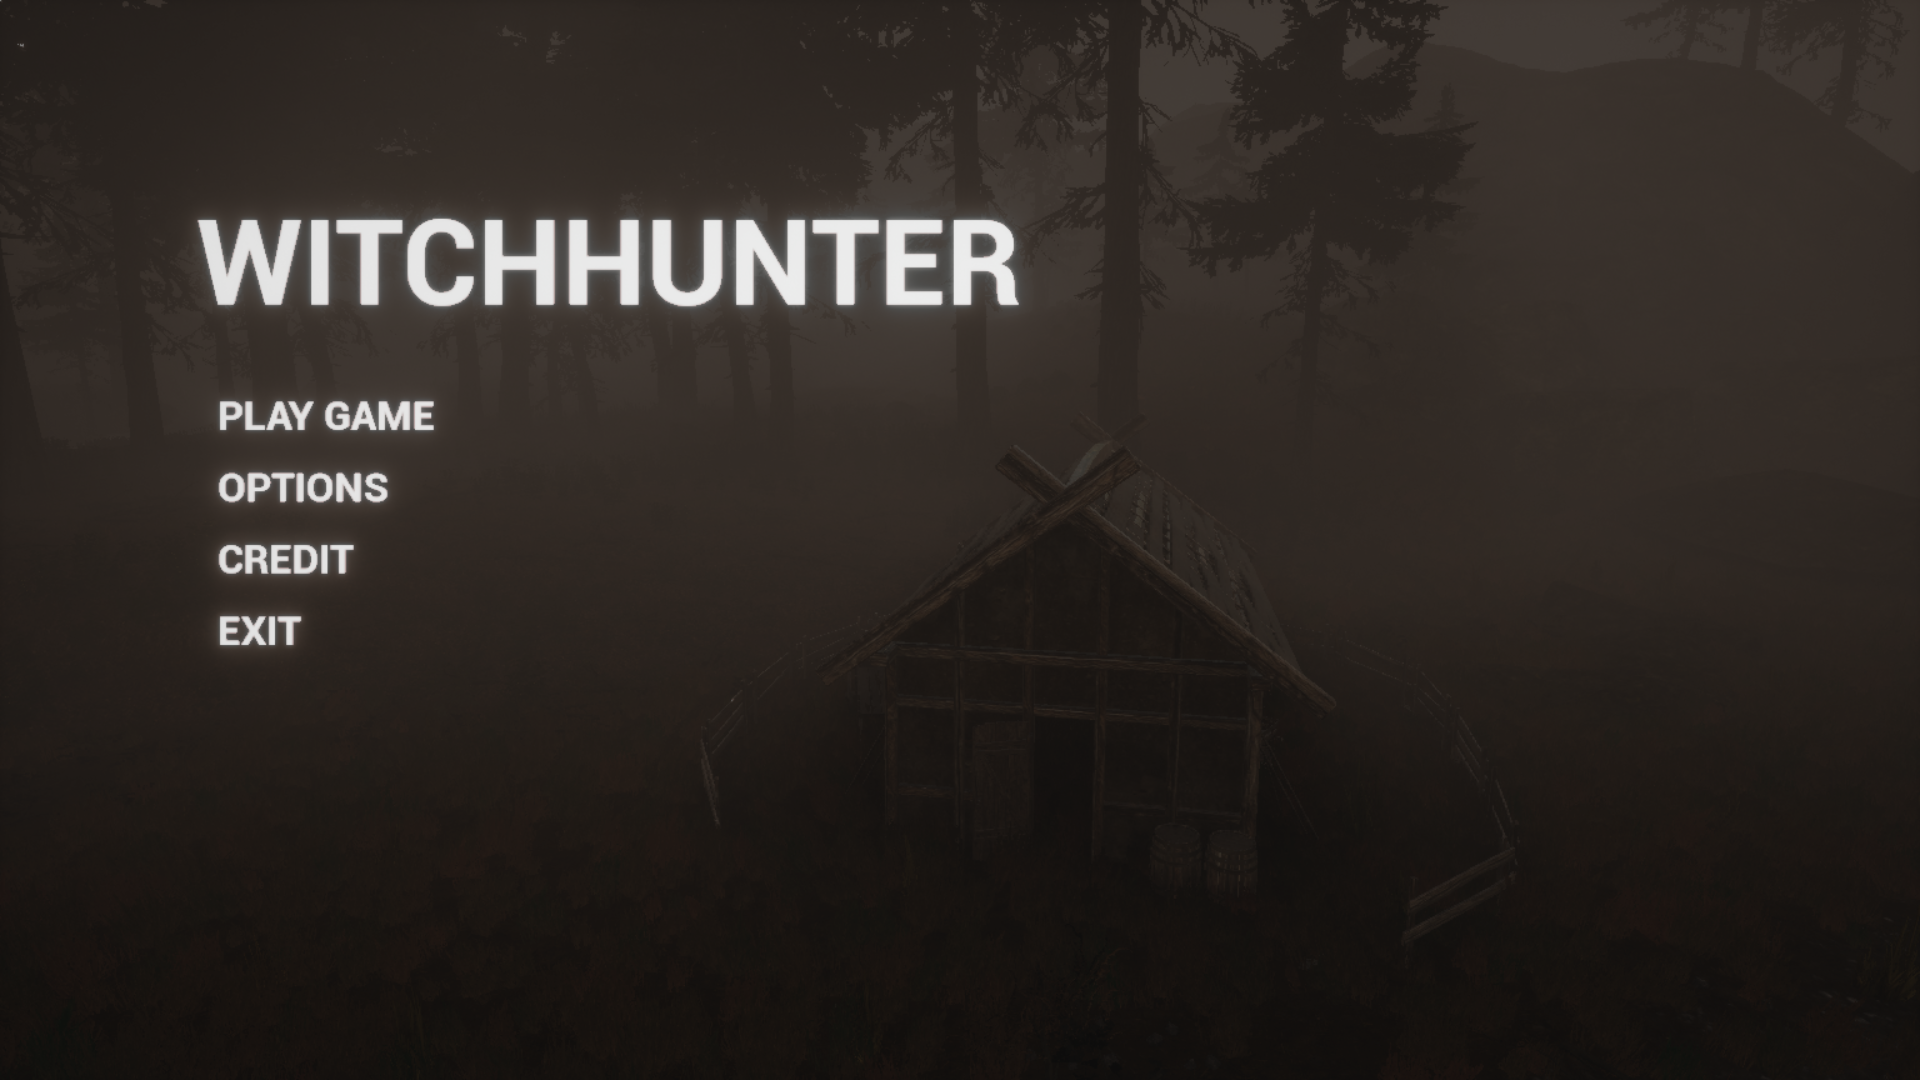
\includegraphics[width=\textwidth]{./img/UI/mainmenu.png}
  \end{center}
  \caption[หน้า Main Menu]{หน้า Main Menu}
  \label{fig:main_menu}
\end{figure}

\pagebreak

\begin{figure}[h!]
  \begin{center}
  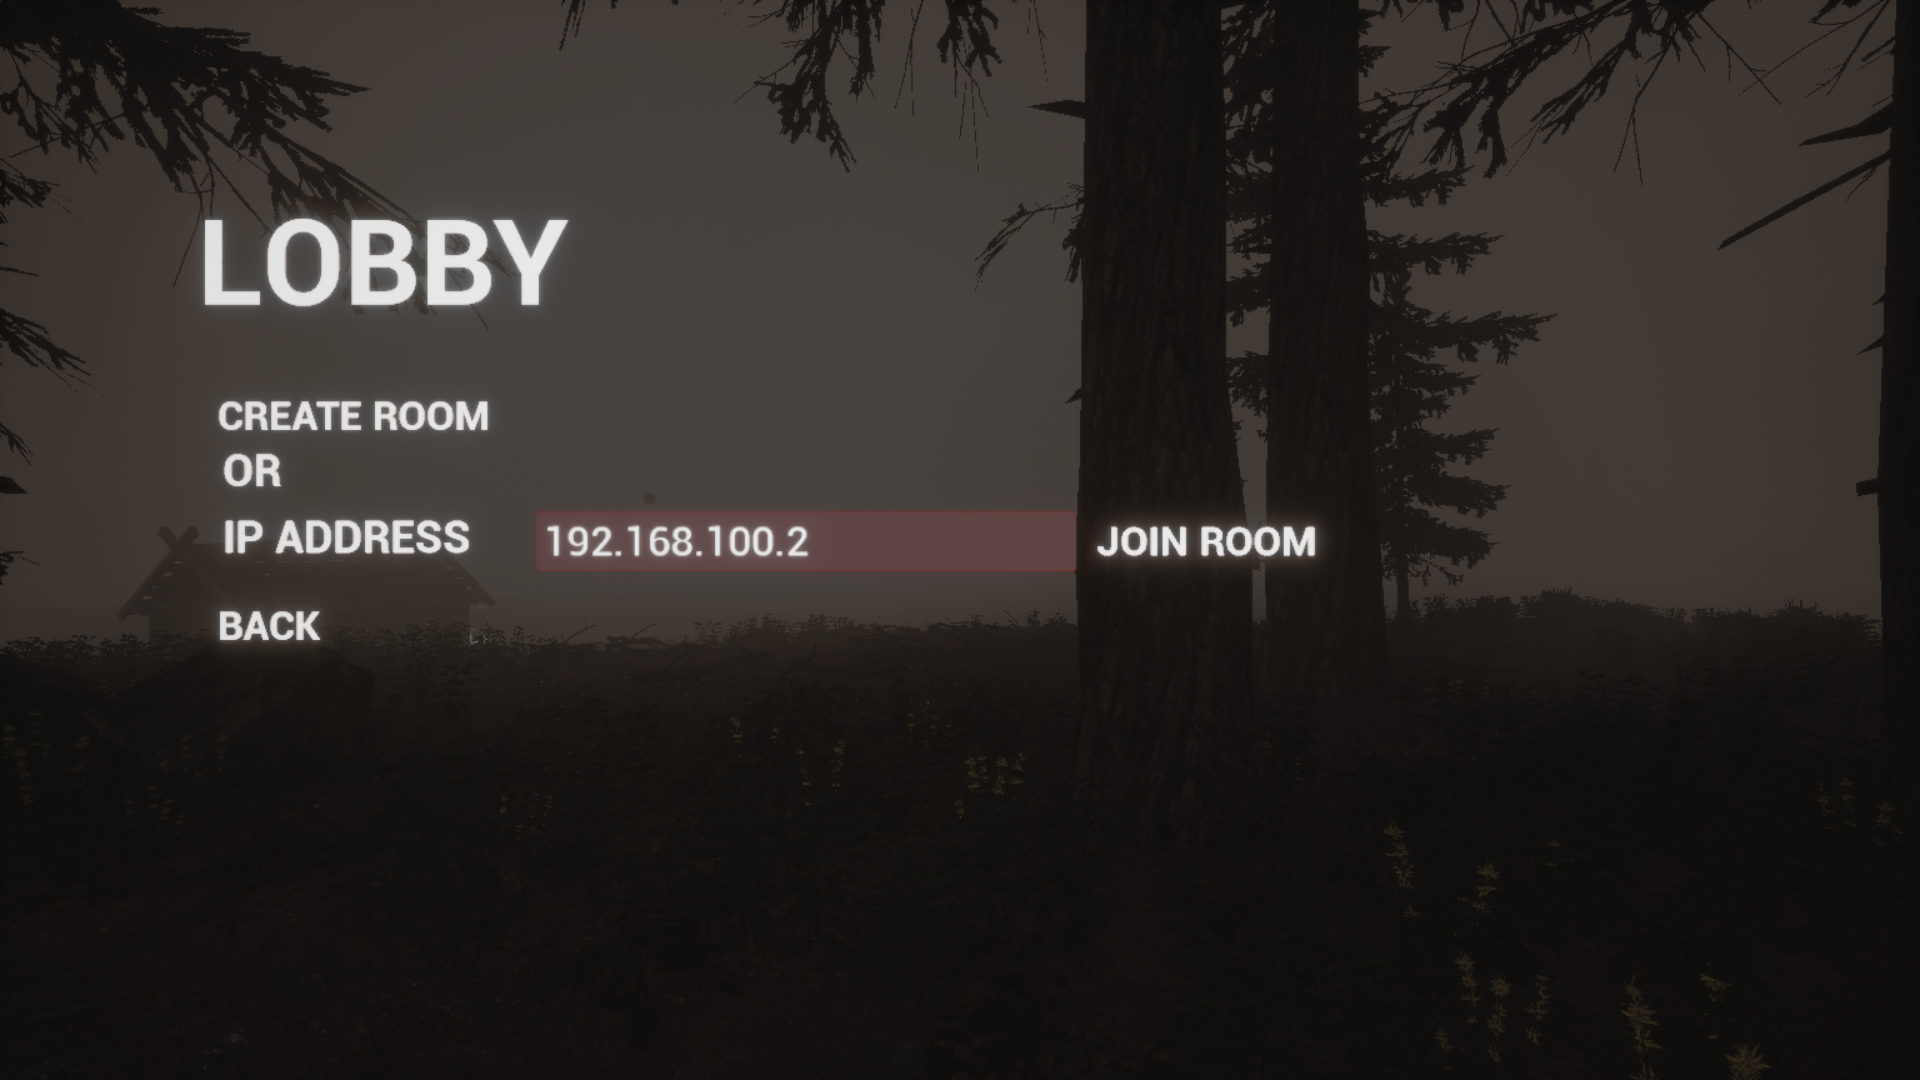
\includegraphics[width=\textwidth]{./img/UI/create_room.png}
  \end{center}
  \caption[หน้าสร้างห้องหรือเข้าร่วมห้อง]{หน้าสร้างห้องหรือเข้าร่วมห้อง}
  \label{fig:create_room}
\end{figure}

\begin{figure}[h!]
  \begin{center}
  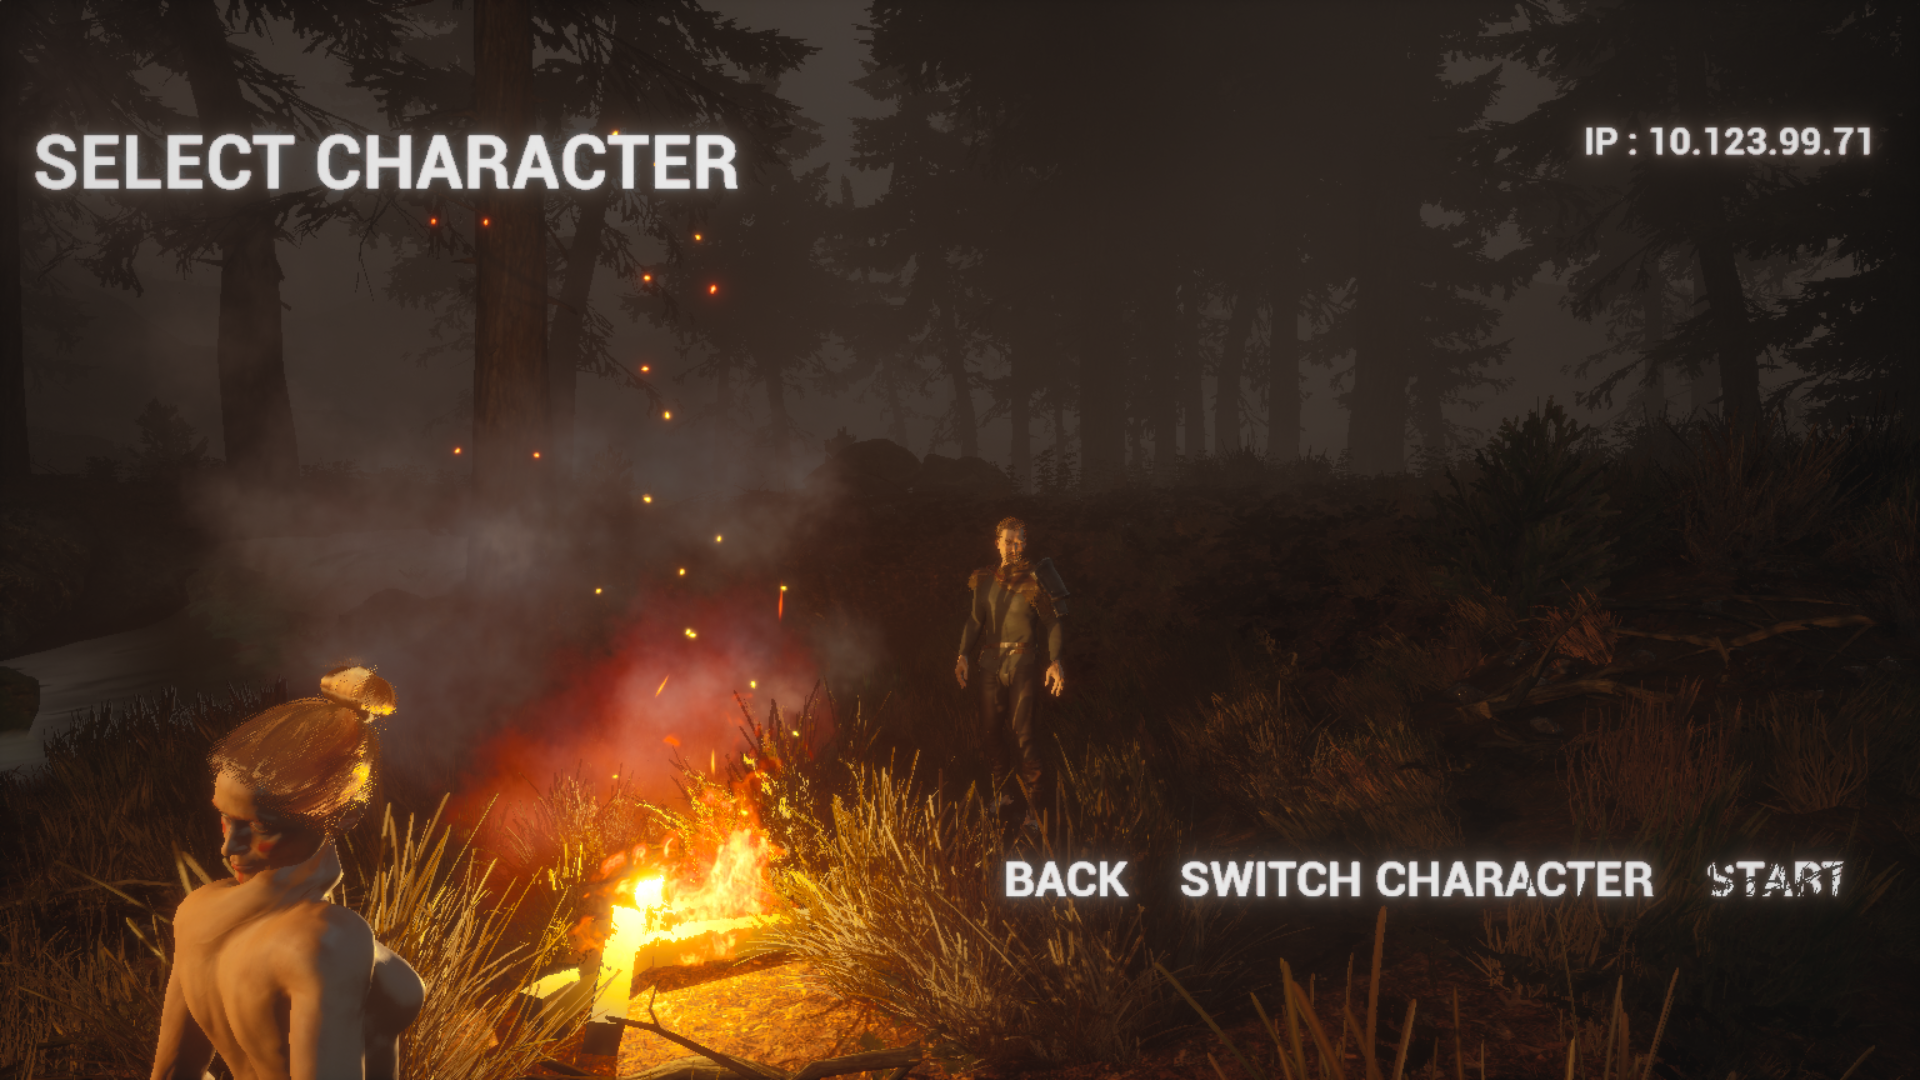
\includegraphics[width=\textwidth]{./img/UI/select_character.png}
  \end{center}
  \caption[หน้าเลือกตัวละครหลังจากเข้าร่วมห้องแล้ว]{ผู้เล่นสามารถเลือกฝ่ายและตัวละครที่อยากเล่นได้ด้วยการกดปุ่ม Switch Character และสามารถเห็นตัวละครของผู้เล่นคนอื่น ๆ}
  \label{fig:select_character}
\end{figure}

\subsubsection{UI ของฝ่าย Hunters}

ด้านบนซ้ายแสดงสถานะของเกม หลอด Circular Progress Bar แสดงเวลาในการทำภารกิจที่ยังเหลืออยู่ ถัดมาบอกจำนวนครั้งของพิธีที่ได้ทำไปแล้ว
ด้านล่างซ้ายแสดงเมนู Inventory

\begin{figure}[h]
  \begin{center}
  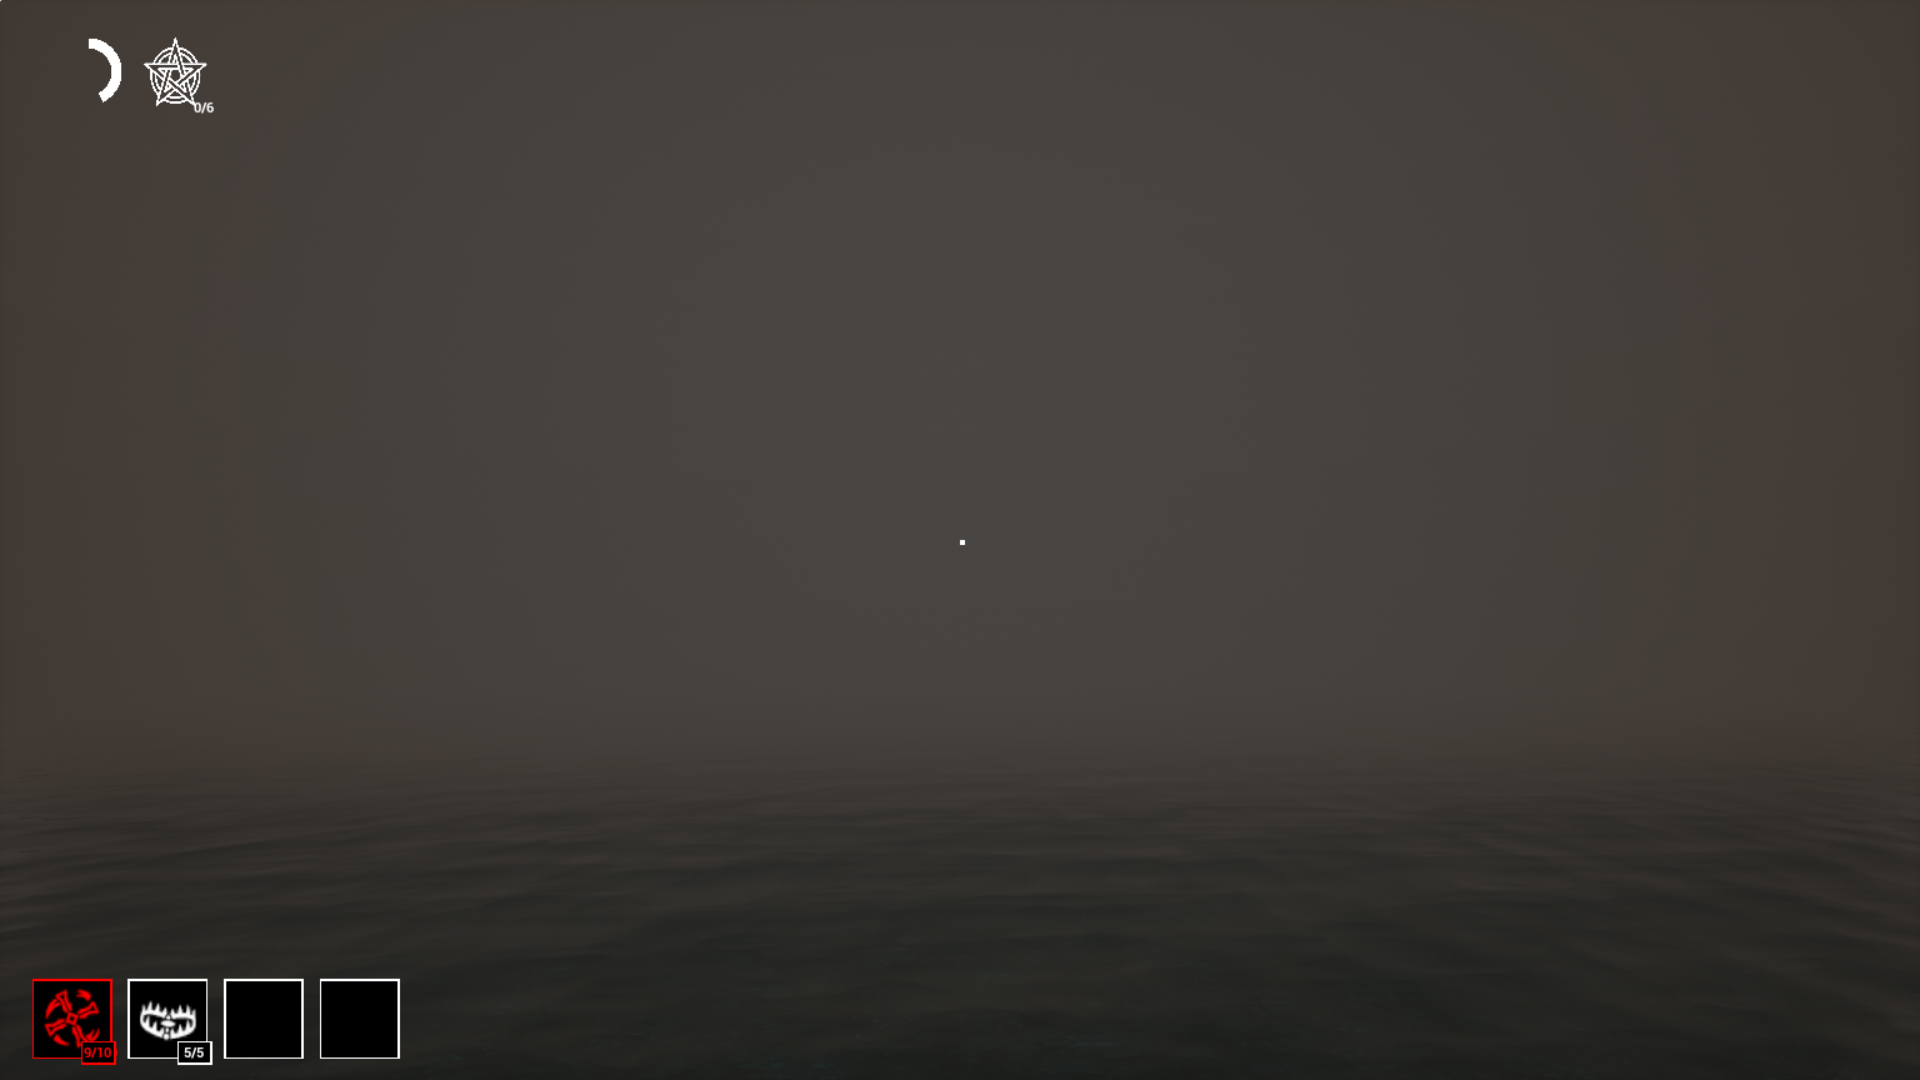
\includegraphics[width=0.8\textwidth]{./img/UI/hunter_ui.png}
  \end{center}
  \caption[ภาพ User Interface ของ Hunter]{ภาพ User Interface ของ Hunter}
  \label{fig:hunter_ui}
\end{figure}

\subsubsection{UI ของฝ่าย Witch}

ด้านบนซ้ายแสดงสถานะของเหมือนกับของ Hunter ด้านล่างซ้ายแสดงสถานะของความสามารถพิเศษที่สามารถสิงกวางได้ บอกถึงคูลดาวน์ของพลัง

\begin{figure}[h]
  \begin{center}
  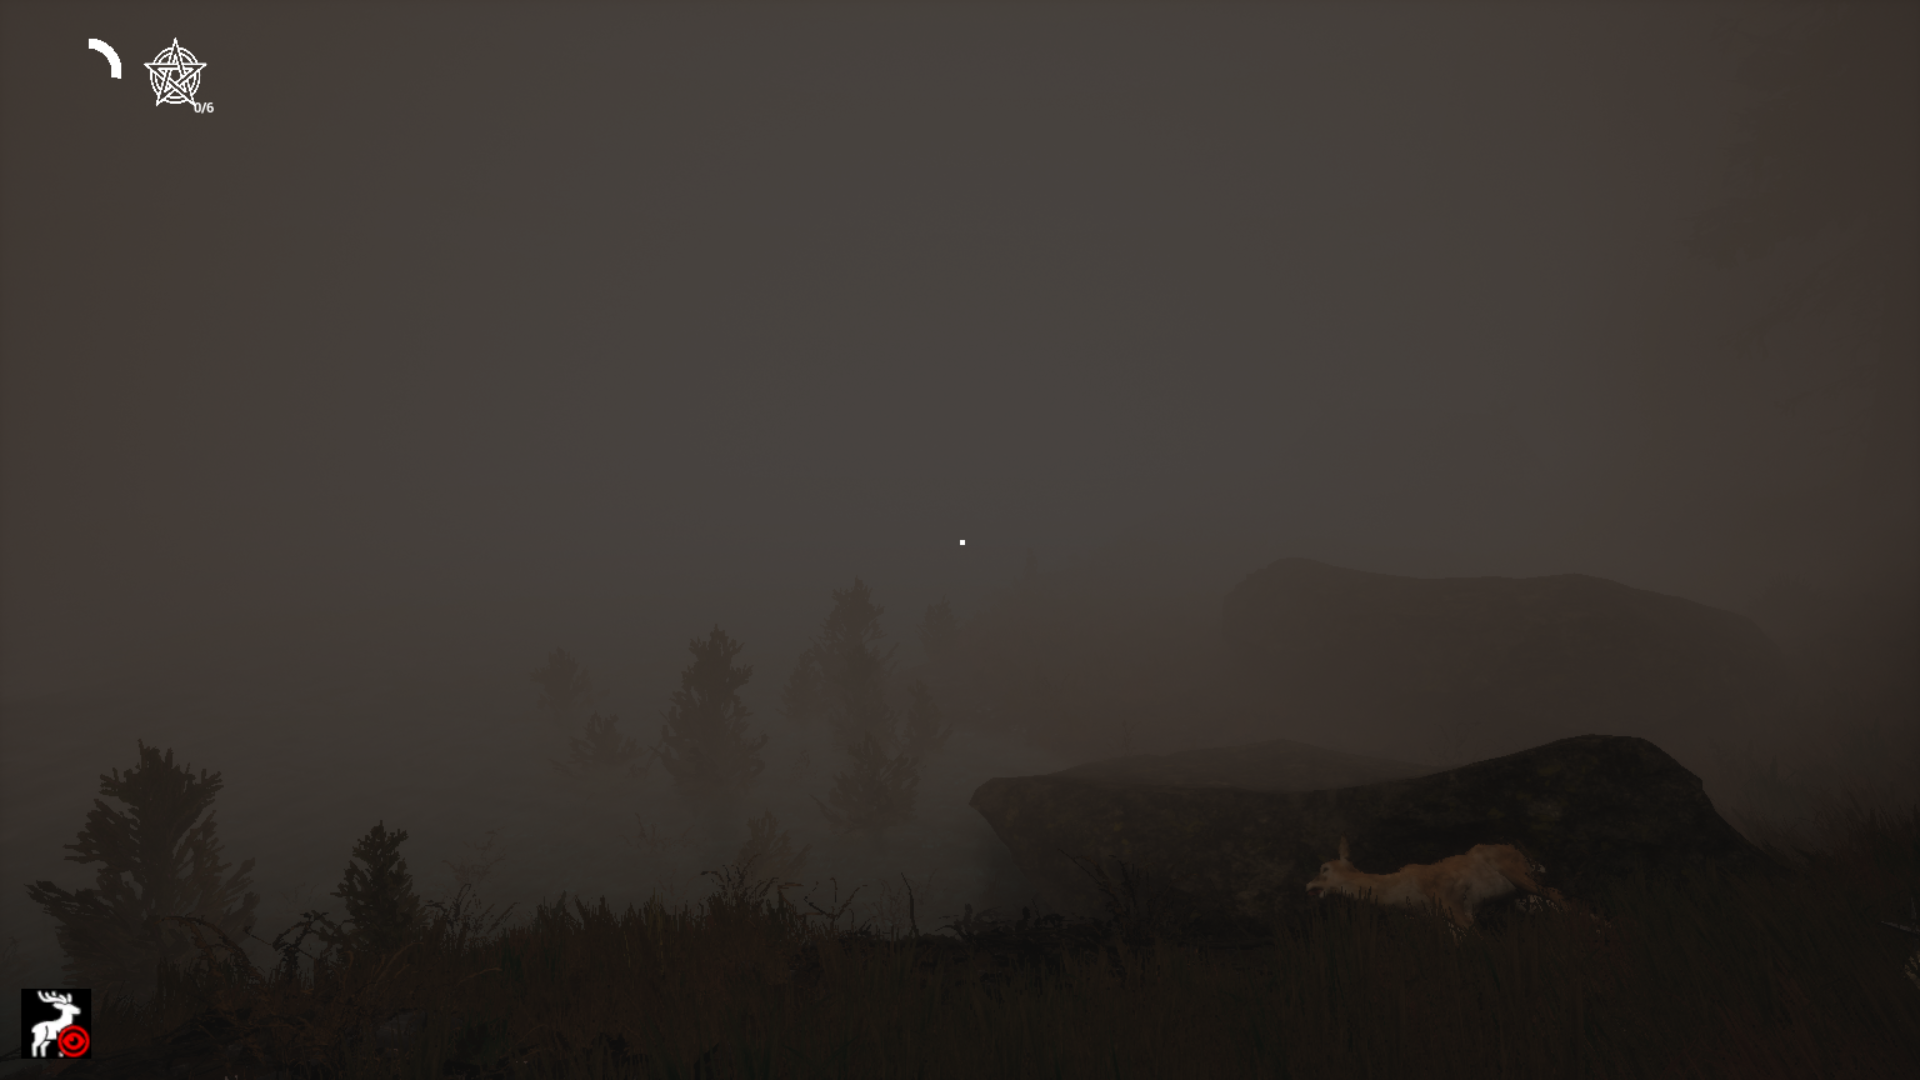
\includegraphics[width=0.8\textwidth]{./img/UI/witch_ui.png}
  \end{center}
  \caption[ภาพ User Interface ของ Witch]{ภาพ User Interface ของ Witch}
  \label{fig:witch_ui}
\end{figure}
\chapter{\ifproject%
\ifenglish Experimentation and Results\else การทดลองและผลลัพธ์\fi
\else%
\ifenglish System Evaluation\else การประเมินระบบ\fi
\fi}
\section{วัตถุประสงค์ของการทดสอบ}
\begin{enumerate}
    \item ทดสอบว่าผู้เล่นได้รับความสนุกสนานจากการเล่นเกม Witch Hunter
    \item ทดสอบการทำงานของระบบเกมว่าถูกต้องสมบูรณ์
\end{enumerate}
\section{การทดสอบความพึงพอใจในการเล่น}

ผู้พัฒนาได้ทดสอบเกมกับผู้เล่นจำนวน 10 คนในช่วงอายุ 20-23 ปี ซึ่งส่วนใหญ่เป็นผู้ที่คุ้นเคยกับการเล่นเกม Multiplayer Action-Horror
โดยให้ผู้เล่นจับกลุ่มกันและสลับบทบาทกันเล่น รวมถึงมีการสลับกลุ่มคละ ๆ กันระหว่างผู้ที่ชำนาญและไม่ชำนาญในการเล่นเกมนี้
ทั้งหมดนี้ก็เพื่อให้ได้ประสบการณ์เล่นที่ครบถ้วนและทดสอบความสมดุลของแต่ละฝั่งในเกม คะแนนความพึงพอใจในเล่นเกมมี 5 ระดับ:
1.ไม่พอใจที่สุด 2.ไม่พอใจ 3.พอใจ 4.พอใจมาก 5.พอใจมากที่สุด  ซึ่งผลลัพธ์ของการทดสอบความพึงพอใจเป็นดังนี้

\begin{figure}[h]
\begin{subfigure}{\textwidth}
    \begin{center}
    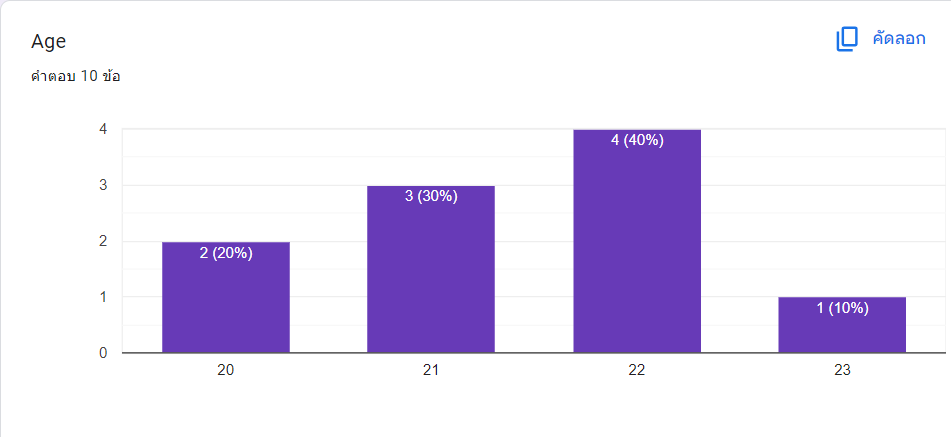
\includegraphics[width=0.8\textwidth]{./img/result/1.png}
    \label{fig:age}
    \end{center}
\end{subfigure}
\begin{subfigure}{\textwidth}
    \begin{center}
    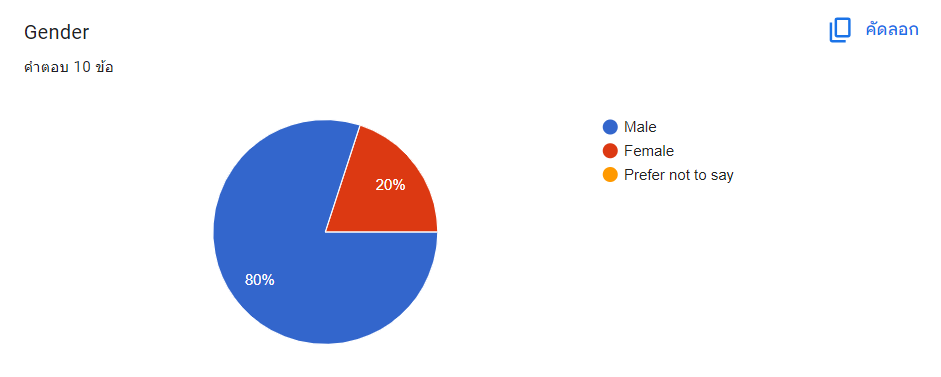
\includegraphics[width=0.8\textwidth]{./img/result/2.png}
    \label{fig:gender}
    \end{center}
\end{subfigure}
\caption{กราฟแสดงอายุและเพศของผู้เข้าร่วมการทดสอบ}
\end{figure}

\begin{figure}[h]
\begin{subfigure}{\textwidth}
    \begin{center}
    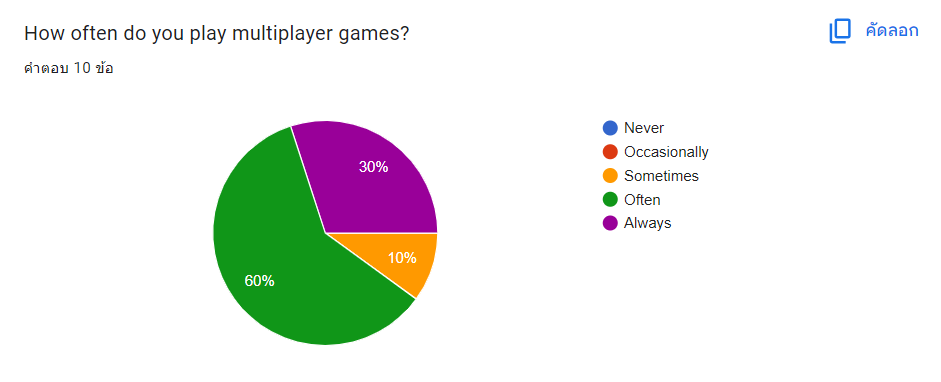
\includegraphics[width=0.8\textwidth]{./img/result/3.png}
    \end{center}
\end{subfigure}
\begin{subfigure}{\textwidth}
    \begin{center}
    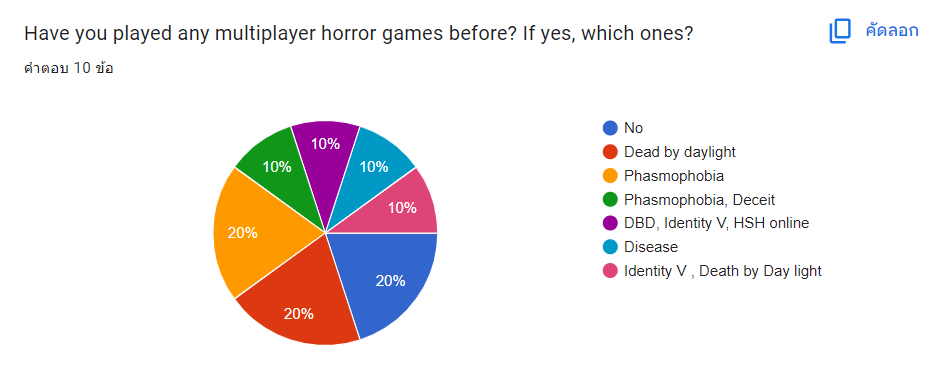
\includegraphics[width=0.8\textwidth]{./img/result/4.png}
    \end{center}
\end{subfigure}
\caption{กราฟแสดงข้อมูลประวัติการเล่นเกมแนว Multiplayer Horror ของผู้เข้าร่วมการทดสอบ}
\end{figure}

\begin{table}[]
    \begin{tabular}{|p{0.65\textwidth}|lllllr|}
    \hline
    \multicolumn{1}{|c|}{\multirow{2}{*}{คำถาม}} &
      \multicolumn{5}{c|}{ระดับการวัดผล} &
      \multicolumn{1}{c|}{\multirow{2}{*}{ค่าเฉลี่ย}} \\ \cline{2-6}
    \multicolumn{1}{|c|}{} &
      \multicolumn{1}{c|}{1} &
      \multicolumn{1}{c|}{2} &
      \multicolumn{1}{c|}{3} &
      \multicolumn{1}{c|}{4} &
      \multicolumn{1}{c|}{5} &
      \multicolumn{1}{c|}{} \\ \hline
    How immersive did you find the game? &
      \multicolumn{1}{c|}{0} &
      \multicolumn{1}{c|}{0} &
      \multicolumn{1}{c|}{5} &
      \multicolumn{1}{c|}{3} &
      \multicolumn{1}{l|}{1} &
      3.56 \\ \hline
    How would you rate your overall enjoyment of the multiplayer horror game? &
      \multicolumn{1}{l|}{0} &
      \multicolumn{1}{l|}{0} &
      \multicolumn{1}{l|}{3} &
      \multicolumn{1}{l|}{7} &
      \multicolumn{1}{l|}{0} &
      3.70 \\ \hline
    How effective were the game's mechanics in creating a sense of tension and fear? &
      \multicolumn{1}{l|}{0} &
      \multicolumn{1}{l|}{2} &
      \multicolumn{1}{l|}{2} &
      \multicolumn{1}{l|}{4} &
      \multicolumn{1}{l|}{2} &
      3.60 \\ \hline
    How well did the game utilize sound effects and music to enhance the horror experience? &
      \multicolumn{1}{l|}{0} &
      \multicolumn{1}{l|}{0} &
      \multicolumn{1}{l|}{1} &
      \multicolumn{1}{l|}{5} &
      \multicolumn{1}{l|}{4} &
      4.30 \\ \hline
    How would you rate the graphical quality and visual atmosphere of the game? &
      \multicolumn{1}{l|}{0} &
      \multicolumn{1}{l|}{0} &
      \multicolumn{1}{l|}{2} &
      \multicolumn{1}{l|}{4} &
      \multicolumn{1}{l|}{4} &
      4.20 \\ \hline
    Considering all aspects of the game, how likely are you to recommend it to a friend? &
      \multicolumn{1}{l|}{0} &
      \multicolumn{1}{l|}{1} &
      \multicolumn{1}{l|}{4} &
      \multicolumn{1}{l|}{4} &
      \multicolumn{1}{l|}{1} &
      3.50 \\ \hline
    How satisfied were you with the pacing of the game? &
      \multicolumn{1}{l|}{0} &
      \multicolumn{1}{l|}{1} &
      \multicolumn{1}{l|}{5} &
      \multicolumn{1}{l|}{3} &
      \multicolumn{1}{l|}{1} &
      3.40 \\ \hline
    \textbf{คะแนนเฉลี่ยความพึงพอใจ} &
      \multicolumn{6}{r|}{3.75} \\ \hline
    \end{tabular}
    \caption{คะแนนจากการทดสอบความพึงพอใจในการเล่น}
\end{table}

\pagebreak

\textbf{ตัวอย่างความคิดเห็นเรื่องความรู้สึกขณะเล่นเกม}
\begin{enumerate}
    \item "บรรยากาศชวนระแวง แต่ก็สนุกและก็ลุ้นดี ตัวละครชวนน่ากลัวเข้ากับเกม"
    \item "Witch - รู้สึกสนุกดีแต่ว่าท่าอ้วกใช้ยากมาก ไม่เคยโดน เดินไปแทบจะจูบ hunter แล้วก็ยังไม่โดน
    Hunter - รู้สึกว่าการทำ objective ไม่ได้ยากเกินไป แต่ว่าตอนสวดทำพิธีนานไปมากๆ ควรลดเวลาลงหน่อย"
    \item "ตื่นเต้นดี งงๆ ตอนแรก แต่ถ้าเล่นไปน่าจะสนุกขึ้น"
    \item "Hunter: ระทึกดีโดยเฉพาะตอนโดน witch ไล่ เกมเพลย์ต้องใช้ความสามารถระดับนึง เช่น การปามีด
    Witch: ค่อนข้างเก่ง โดยเฉพาะท่าชาร์จยิงคลิกขาว ท่าคลิกซ้ายใช้งานยาก"
\end{enumerate}

\textbf{ตัวอย่างความคิดเห็นเรื่องสิ่งที่อยากให้ปรับปรุง}
\begin{enumerate}
    \item "มีให้เห็นว่าเพื่อนเราโดนตีกี่ที ใกล้ตายรึยัง สถานะเป็นยังไง "
    \item "มีแมพเล็กๆ  ให้ดูมุมซ้ายบน"
    \item "ในอนาคตอาจจะมีจำนวนตัวละครในแต่ละเกมเพิ่ม"
    \item "สกิลเฉพาะแต่ละตัวละคร"
    \item "ฮันเตอร์กับวิชน่าจะจับคู่แบบห้องที่ไม่เห็นตัวละครต่างฝ่ายกัน "
    \item "มีข้อความกดบอกกันว่าวิชอยู่ใกล้ หรือ ทำอะไรอยู่เป็นต้น"
\end{enumerate}

จากผลการทดสอบ ผู้เล่นมีความพอใจมากที่สุดในเรื่องของเสียงและเพลงประกอบเกมที่ช่วยสร้างเสริมประสบการณ์ที่ระทึกและสยองขวัญ
โดยมีคะแนนเฉลี่ยอยู่ที่ 4.30 จาก 5 ส่วนที่ควรมีการปรับปรุงมากที่สุดคือเรื่องจังหวะของเกม (Pacing) 
ซึ่งมีคะแนนเฉลี่ยอยู่ที่ 3.40 อยู่ในระดับพอใจ ในเรื่องของความสนุกสนานของเกมและการสร้างความตึงเครียดและสยองขวัญให้กับผู้เล่น
มีคะแนนเฉลี่ยอยู่ที่ 3.70 และ 3.60 ตามลำดับ โดยรวมแล้วผู้เล่นมีความพึงพอใจในการเล่นเกม Witch Hunter อยู่ที่ 3.75 จาก 5 อยู่ในระดับพอใจค่อนไปทางพอใจมาก
สรุปได้ว่าเกมนี้จะดีขึ้นอีกถ้ามีการปรับปรุงเรื่องของจังหวะของเกมให้เหมาะสมมากขึ้น ปรับปรุงการใช้งานสกิลให้ตัวละครให้ง่ายขึ้น และแก้ไขข้อบกพร่องต่าง
 ๆ ในระบบเกมที่เกิดขึ้นบางครั้งในระหว่างการทดสอบ

\ifproject
\chapter{\ifenglish Conclusions and Discussions\else บทสรุปและข้อเสนอแนะ\fi}

\section{\ifenglish Conclusions\else สรุปผล\fi}

จากการทดสอบเล่นเกม Witch Hunter พบว่าผู้เล่นมีความสนุกสนานในการเล่นเกม และมีความพึงพอใจในการเล่นเกมค่อนข้างมาก
รู้สึกพอใจอย่างมากกับเสียงประกอบและกราฟิกที่สมจริง เป็นอันว่าบรรลุวัตถุประสงค์ของโครงงานนี้

\section{\ifenglish Challenges\else ปัญหาที่พบและแนวทางการแก้ไข\fi}

ในการทำโครงงานนี้ พบว่าเกิดปัญหาหลักๆ ดังนี้
\begin{enumerate}
    \item ความบกพร่องที่เกิดจากความเสถียรของเครือข่ายอินเตอร์เน็ตที่ถูกค้นพบตอนทดสอบเล่นจริง ๆ เท่านั้น 
    และต้องอาศัยความรู้เรื่องระบบ Multiplayer ใน Unreal Engine รวมถึงต้องคำนึงเรื่อง Lag Compensation, 
    Package Loss และ Race Condition ทั้งหมดนี้ทำให้การพัฒนาเกมล่าช้ากว่าที่คาดหวัง
    \item ผู้พัฒนามีประสบการณ์น้อยในการพัฒนาเกมโดยเฉพาะกับ Unreal Engine ส่งผลให้การพัฒนาระบบของเกมล่าช้า 
    และมีข้อผิดพลาดในการออกแบบการเล่นของเกม
\end{enumerate}

\section{\ifenglish%
Suggestions and further improvements
\else%
ข้อเสนอแนะและแนวทางการพัฒนาต่อ
\fi
}

ข้อเสนอแนะเพื่อพัฒนาโครงงานนี้ต่อไป มีดังนี้
\begin{enumerate}
    \item ปรับปรุงจังหวะของเกม เช่น เวลาการทำภารกิจหลัก ให้มีความระทึกและสนุกสนานมากยิ่งขึ้น
    \item ปรับปรุงการควบคุมให้ง่ายขึ้น ทำให้ผู้เล่นใช้สกิลและเล่นเกมได้ง่ายขึ้น
    \item เพิ่มจำนวนตัวละครและสกิลเพื่อเพิ่มความหลากหลายในการเล่น
    \item ปรับปรุงประสิทธิภาพของเกมให้เหมาะสมกับเครื่องที่มีสเปคต่ำ ทั้งเรื่องกราฟิก และการทำงานของ
    ระบบเครือข่าย
    \item เพิ่มระบบที่ทำให้การเล่นสะดวกและน่าสนใจมากขึ้น เช่น แผนที่ การแจ้งเตือนเมื่อผู้เล่นอีกคนถูกโจมตี สถานะของผู้เล่นคนอื่น ๆ ระบบปีนป่าย
\end{enumerate}

\fi

\bibliographystyle{plainurl}
\bibliography{report}

\ifproject
\normalspacing
\appendix
\chapter{The first appendix}

วิดีโอบันทึกการเล่นเกมจากการทดสอบ

\section{Appendix section}

็Hunter's Gameplay Video: in progress... \\
Witch's Gameplay Video: in progress...

\chapter{\ifenglish Manual\else คู่มือการใช้งานระบบ\fi}

Manual is in progress...


%% Display glossary (optional) -- need glossary option.
\ifglossary\glossarypage\fi

%% Display index (optional) -- need idx option.
\ifindex\indexpage\fi

\begin{biosketch}
  \begin{center}
    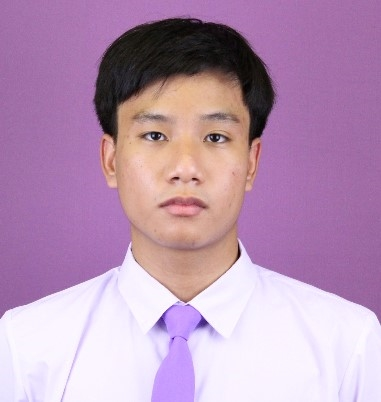
\includegraphics[width=1.5in]{./img/phu.png}
  \end{center}
  \textbf{นายธนดล เดชประภากร} Tanadol Deachprapakorn \\
  \textbf{รหัสนักศึกษา}: 630610734 \\
  \textbf{อีเมล}: \href{mailto:tanadol-de@outlook.com}{tanadol-de@outlook.com}
  \begin{itemize}
    \item เข้าร่วม Global Game Jam 2023 ที่เชียงใหม่
    \item เข้าร่วม The 3rd Kibo Robot Programming Challenge 2022 จัดโดย สำนักงานพัฒนาวิทยาศาสตร์และเทคโนโลยีแห่งชาติ(สวทช.) และองค์การสำรวจอวกาศญี่ปุ่น (JAXA) - ได้รับรางวัล Top 20th Finalist เป็นผู้ชนะเลิศอันดับที่ 4
    \item	เข้าร่วม Faipa Hackathon วิเคราะห์และบริหารวิกฤตการณ์ไฟป่าด้วยเทคโนโลยีดาวเทียมและ Big Data – ได้รับรางวัลรองชนะเลิศอันดับที่ 2 ร่วมคิดการบูรณการ Hotspot, sensor, การสื่อสาร วิธีการรับมือไฟป่า
    \item	เข้าร่วมโครงการพัฒนาระบบนิเวศเพื่อสร้างผู้ประกอบการรุ่นใหม่ (Entrepreneurial Ecosystem Development) จัดโดย อุทยานวิทยาศาสตร์และเทคโนโลยี มหาวิทยาลัยเชียงใหม่
    \item เข้าร่วม สู้ (ทัน) ควัน 32hrs. Hackathon นวัตกรรม สู้หมอกควัน - ได้รับรางวัลชนะเลิศอันดับที่ 1 ร่วมคิดการตรวจจับไฟป่า และแจ้งเตือน โดยใช้อากาศยานไร้คนขับ
    \item เข้าร่วมโครงการเสวนาวิชาการและแข่งขัน Hackathon การมีส่วนร่วมของประชาชนในการแก้ไขรัฐธรรมนูญและเสนอนโยบาย ครั้งที่ 1 – ได้รับรางวัลชนะเลิศอันดับ 1 ประเภทแพลตฟอร์มออนไลน์ ร่วมคิดแพลตฟอร์มออนไลน์ในการเสนอกฎหมาย
  \end{itemize}
\end{biosketch}

\begin{biosketch}
  \begin{center}
    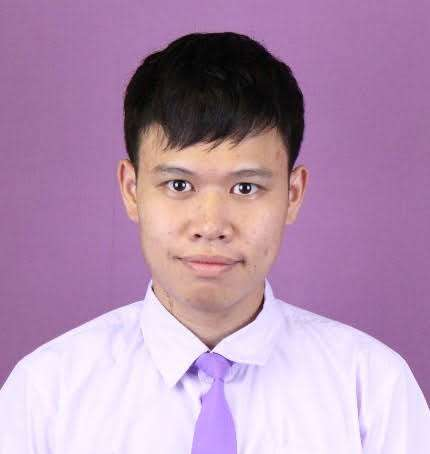
\includegraphics[width=1.5in]{./img/rich.png}
  \end{center}
  \textbf{นายภูริช สีนวลแล} Purich Seenaullae \\
  \textbf{รหัสนักศึกษา}: 630610752 \\
  \textbf{อีเมล}: \href{mailto:purich_s@cmu.ac.th}{purich\_s@cmu.ac.th}
  \begin{itemize}
    \item เข้าร่วม Global Game Jam 2023 ที่เชียงใหม่
    \item	เข้าร่วมโครงการพัฒนาระบบนิเวศเพื่อสร้างผู้ประกอบการรุ่นใหม่ (Entrepreneurial Ecosystem Development) จัดโดย อุทยานวิทยาศาสตร์และเทคโนโลยี มหาวิทยาลัยเชียงใหม่
    \item เข้าร่วม สู้ (ทัน) ควัน 32hrs. Hackathon นวัตกรรม สู้หมอกควัน - ได้รับรางวัลชนะเลิศอันดับที่ 1 ร่วมคิดการตรวจจับไฟป่า และแจ้งเตือน โดยใช้อากาศยานไร้คนขับ
    \item เข้าร่วมโครงการเสวนาวิชาการและแข่งขัน Hackathon การมีส่วนร่วมของประชาชนในการแก้ไขรัฐธรรมนูญและเสนอนโยบาย ครั้งที่ 1 – ได้รับรางวัลชนะเลิศอันดับ 1 ประเภทแพลตฟอร์มออนไลน์ ร่วมคิดแพลตฟอร์มออนไลน์ในการเสนอกฎหมาย
  \end{itemize}
\end{biosketch}
\fi % \ifproject
\end{document}
